\documentclass[12pt,a4paper,bibliography=totocnumbered,listof=totocnumbered]{scrartcl}
% u.U. muss Koma-Skript Package ueber MikTeX deinstalliert und neu installiert werden
% Hilft das nicht, so sollte statt scrartcl die Dokumentenklasse article verwendet werden
%\usepackage[backend=bibtex,style=alphabetic]{biblatex}
%\usepackage[backend=bibtex,style=ieee]{biblatex}
\usepackage[style=ieee]{biblatex}
\usepackage[ngerman]{babel}
\usepackage[utf8]{inputenc}
\usepackage{ifthen}
\usepackage{xargs}
\usepackage{amsmath}
\usepackage{amsfonts}
\usepackage{amssymb}
\usepackage{graphicx}
\usepackage{caption}
\usepackage{fancyhdr}
\usepackage{tabularx}
\usepackage{geometry}
\usepackage{setspace}
\usepackage[right]{eurosym}
\usepackage[printonlyused]{acronym}
\usepackage{subfig}
\usepackage{floatflt}
\usepackage[usenames,dvipsnames]{color}
\usepackage{colortbl}
\usepackage{paralist}
\usepackage{array}
\usepackage{titlesec}
\usepackage{parskip}
\usepackage[right]{eurosym}
\usepackage[subfigure,titles]{tocloft}
%\usepackage[pdfpagelabels=true]{hyperref}
\usepackage[pdfpagelabels=true]{hyperref}

\usepackage{listings}
\lstset{basicstyle=\footnotesize, captionpos=b, breaklines=true, showstringspaces=false, tabsize=2, frame=lines, numbers=left, numberstyle=\tiny, xleftmargin=2em, framexleftmargin=2em}
\makeatletter
\def\l@lstlisting#1#2{\@dottedtocline{1}{0em}{1em}{\hspace{1,5em} Lst. #1}{#2}}
\makeatother

%\geometry{a4paper, top=27mm, left=20mm, right=20mm, bottom=35mm, headsep=10mm, footskip=12mm}

\definecolor{javared}{rgb}{0.6,0,0} % for strings
\definecolor{javagreen}{rgb}{0.25,0.5,0.35} % comments
\definecolor{javapurple}{rgb}{0.5,0,0.35} % keywords
\definecolor{javadocblue}{rgb}{0.25,0.35,0.75} % javadoc
\definecolor{gray}{rgb}{0.6,0.6,0.6}
 
\lstset{language=Java,
basicstyle=\ttfamily\footnotesize,
keywordstyle=\color{javapurple}\bfseries,
stringstyle=\color{javared},
commentstyle=\color{javagreen}\itshape\bfseries,
morecomment=[s][\color{javadocblue}]{/**}{*/},
numbers=left,
numberstyle=\tiny\color{gray},
stepnumber=1,
numbersep=10pt,
tabsize=3,
showspaces=false,
showstringspaces=false}
\titlespacing{\section}{0pt}{12pt plus 4pt minus 2pt}{-6pt plus 2pt minus 2pt}

% Kopf- und Fusszeile
\renewcommand{\sectionmark}[1]{\markright{#1}}
\renewcommand{\leftmark}{\rightmark}
\pagestyle{fancy}
\lhead{}
\chead{}
\rhead{\thesection\space\contentsname}
\lfoot{}
\cfoot{}
\rfoot{\ \linebreak Seite \thepage}
\renewcommand{\headrulewidth}{0.4pt}
\renewcommand{\footrulewidth}{0.4pt}

% Vorspann
\renewcommand{\thesection}{\Roman{section}}
\renewcommand{\theHsection}{\Roman{section}}
\pagenumbering{Roman}

\newcommand{\folgen}[1]{
\ensuremath
#1
}

\newcommandx{\student}[3][]{
	\def\studentName{#1}%
	\def\studentMatnr{#2}%
	\def\studentStudiengang{#3}%
}

\newcommandx{\MyTitelseite}[8][]{
\thispagestyle{empty}

\includegraphics[scale=0.2]{pics/oth-logo.png}%\hfill\includegraphics[scale=0.5]{#1}
\begin{center}
\ifthenelse{\equal{#2}{2}}{ % then
	\vspace*{2cm}
	\Large
	\textbf{Ostbayerische Technische Hochschule Regensburg}\\
	\textbf{Fakultät für Informatik und Mathematik}\\
	\vspace*{2cm}
	\Huge
	\textbf{#3}\\[1em]
	\large
	Zur Erlangung des akademischen Grades des\\
	\ifthenelse{\equal{#3}{Bachelorarbeit}}{Bachelor of Science (B.Sc.)}{Master of Science (M.Sc.)}\\
	\vspace*{1cm}
	\Large
	\textbf{#4}\\
}{ % else
	\vspace*{1cm}
	\Large
	\textbf{#4}\\
	\vspace*{2cm}
	\large
	An der Fakultät für Informatik und Mathematik der\\
	Ostbayerischen Technischen Hochschule Regensburg\\
	im Studiengang\\
	\studentStudiengang\\[2em]
	eingereichte\\
	\vspace*{1cm}
	\Large
	\textbf{#3}\\[2em]
	\large
	zur Erlangung des akademischen Grades des\\
	\ifthenelse{\equal{#3}{Bachelorarbeit}}{Bachelor of Science (B.Sc.)}{Master of Science (M.Sc.)}
	\vspace*{1cm}
	\Large
}
	\vfill
	\normalsize
	%\newcolumntype{x}[1]{>{\raggedleft\arraybackslash\hspace{0pt}}p{#1}}
	\begin{tabular}{rl}%{6cm}p{7.5cm}}
	    \rule{0mm}{1ex}\textbf{Vorgelegt von:} & \studentName \\
		\rule{0mm}{1ex}\textbf{Matrikelnummer:} & \hspace*{-0.5em}\begin{tabular}[t]{r}\studentMatnr\end{tabular} \\ 
		\ifthenelse{\equal{#2}{1}}{~\\}{\rule{0mm}{1ex}\textbf{Studiengang:} & \studentStudiengang \\[2em]}
		\rule{0mm}{1ex}\textbf{Erstgutachter:} & #5 \\ 
		\rule{0mm}{1ex}\textbf{Zweitgutachter:} & #6 \\[2em]
		\rule{0mm}{1ex}\textbf{Abgabedatum:} & #7 \\ 
	\end{tabular} 
\end{center}
\pagebreak
}
%\addbibresource{literatur.bib}
\addbibresource{mendeley_v2.bib}


\begin{document}


% ----------------------------------------------------------------------------------------------------------
% Titelseite
% ----------------------------------------------------------------------------------------------------------
\newcommand{\studierenderName}{Philipp Gottschalk}
\student{\studierenderName}		% Studierender
{2853044}						% Matrikelnummer
{Technische Informatik}			% Studiengang

\MyTitelseite{}	% Optionales Logo des extern betreuenden Unternehmens
{1}								% Style der Titelseite (1 oder 2)
{Bachelorarbeit}				% Typ der Abschlussarbeit (\in {Bachelorarbeit, Masterarbeit})
{Analyse und Vergleich von Prozess-Isolationsmechanismen bei Containern und Virtuellen Maschinen}				% Thema der Arbeit						
{Prof.\ Dr.\ Alexander Metzner}		% Betreuer
{Prof.\ Dr.\ Richard Roth}	% Zweitgutachter
{13.10.\the\year}				% Abgabedatum


\thispagestyle{empty}
~\pagebreak

\setcounter{page}{1} 

% ----------------------------------------------------------------------------------------------------------
% Eigensctändigkeitserklaerung
% ----------------------------------------------------------------------------------------------------------
\thispagestyle{empty}
\section*{Erklärung zur Bachelorarbeit}

\bigskip
\bigskip 
\bigskip 

\begin{enumerate}
    \item Mir ist bekannt, dass dieses Exemplar der Bachelorarbeit als Prüfungsleistung in das Eigentum der Ostbayerischen Technischen Hochschule Regensburg übergeht.
    \item Ich erkläre hiermit, dass ich diese Bachelorarbeit selbständig verfasst, noch nicht anderweitig für Prüfungszwecke vorgelegt, keine anderen als die angegebenen Quellen und Hilfsmittel benutzt sowie wörtliche und sinngemäße Zitate als solche gekennzeichnet habe.
\end{enumerate}

\bigskip 
\bigskip 
\bigskip 

Regensburg, den \today

\bigskip 
\bigskip

\line(1,0){200}
\newline
\studierenderName

% ----------------------------------------------------------------------------------------------------------
% Abstract
% ----------------------------------------------------------------------------------------------------------
\thispagestyle{empty}
\setstretch{1.15} % Zeilenspacing
\section*{Zusammenfassung}

\bigskip 


In der folgenden Arbeit wird $\ldots$


% ----------------------------------------------------------------------------------------------------------
% Inhaltsverzeichnis
% ----------------------------------------------------------------------------------------------------------
\tableofcontents
\pagebreak

% ----------------------------------------------------------------------------------------------------------
% Abbildungsverzeichnis
% ----------------------------------------------------------------------------------------------------------
\lhead{}
\rhead{Abbildungsverzeichnis}
\listoffigures
\pagebreak

% ----------------------------------------------------------------------------------------------------------
% Tabellenverzeichnis (optional)
% ----------------------------------------------------------------------------------------------------------
\lhead{}
\rhead{Tabellenverzeichnis}
\listoftables
\pagebreak

% ----------------------------------------------------------------------------------------------------------
% Listingsverzeichnis (optional; Code nur, wenn wirklich sinnvoll und wichtig)
% ----------------------------------------------------------------------------------------------------------
%\lhead{}
%\rhead{Quellcodeverzeichnis}
%\lstlistoflistings
%\pagebreak

% ----------------------------------------------------------------------------------------------------------
% Abkürzungsverzeichnis (optional)
% ----------------------------------------------------------------------------------------------------------
\lhead{}
\rhead{Abkürzungsverzeichnis}
%\listoftables
\section{Abkürzungsverzeichnis}
\begin{acronym}[KDE]
\acro{BA}[BA]{Bachelorarbeit}
\acro{MA}[MA]{Masterarbeit}
\end{acronym}
\pagebreak


% ----------------------------------------------------------------------------------------------------------
% Inhalt
% ----------------------------------------------------------------------------------------------------------
% Abstände Überschrift
\titlespacing{\section}{0pt}{12pt plus 4pt minus 2pt}{0pt plus 2pt minus 2pt}
\titlespacing{\subsection}{0pt}{12pt plus 4pt minus 2pt}{0pt plus 2pt minus 2pt}
\titlespacing{\subsubsection}{0pt}{12pt plus 4pt minus 2pt}{0pt plus 2pt minus 2pt}
%\titlespacing{\Paragraph}{0pt}{12pt plus 4pt minus 2pt}{0pt plus 2pt minus 2pt}
% Kopfzeile
\renewcommand{\sectionmark}[1]{\markright{#1}}
\renewcommand{\subsectionmark}[1]{}
\renewcommand{\subsubsectionmark}[1]{}
%\renewcommand{\paragraphmark}[1]{}

\lhead{Kapitel \thesection}
\rhead{\rightmark}

%\onehalfspacing
\setstretch{1.15}
\renewcommand{\thesection}{\arabic{section}}
\renewcommand{\theHsection}{\arabic{section}}
\setcounter{section}{0}
\pagenumbering{arabic}
\setcounter{page}{1}

\setcounter{secnumdepth}{4}
\titleformat{\paragraph}
{\normalfont\normalsize\bfseries}{\theparagraph}{1em}{}
\titlespacing*{\paragraph}
{0pt}{3.25ex plus 1ex minus .2ex}{1.5ex plus .2ex}

% ----------------------------------------------------------------------------------
% Kapitel: Einleitung
% ----------------------------------------------------------------------------------


\thispagestyle{empty}
\section{Einleitung}
In der Industrie geht es meist darum wie man Kosten einsparen kann. Die Hardware Systeme in Firmen werden häufig nur zu einem geringen Prozentsatz ausgelastet. Neue Hardware für zusätzliche Anforderungen ist sehr teuer. Wenn es nur eine Möglichkeit geben würde auf einem System mehrere voneinander Isolierte Umgebungen zu schaffen und die schon vorhandenen Kapazitäten auszunutzen, könnten kosten durch neue Anschaffung, Platz und sogar Strom gespart werden. Vorallem in der Automobilindustrie geht es bei der Entwicklung von Serienfahrzeugen um möglichst effizient ausgenutzte Räume und Ressourcen. Bereits Cent Beträge die Pro Fahrzeug eingespart werden können, schlagen bei einer Millionenfachen Produktion zu Buche. 

Container als leiftgewichtiger Virtualierung bietet ein 

gegenüberstellung Effizienz Isolierung 
Hardwareaufwand
Ausfallsicherheit 

\subsection{Motivation}
\subsection{Projektbeschreibung}
\subsection{Ziele}

Effiziente ressourcenverteilung 

Überlastung der Hardware
geld sparen 




\pagebreak


% ----------------------------------------------------------------------------------
% Kapitel: Theorie
% ----------------------------------------------------------------------------------

\thispagestyle{empty}

\section{Grundlagen der Virtualisierung}
\label{Grundlagen der Virtualisierung}
Es existieren verschiedenen Ansätze für Virtualisierung, wie zum Beispiel die in dieser Arbeit betrachtete Container- oder Hypervisor-basierte Virtualisierung. Die Virtualisierung wird verwendet, um Hardware effizienter zu nutzen. Dabei wird die Hardware virtuell in kleinere Einheiten zerlegt, die voneinander isoliert sind. Auf diesen Einheiten können Prozesse ausgeführt werden, die nichts von den Prozessen in anderen Einheiten wissen. Dabei ist vor allem die Isolierung dieser Einheiten von Interesse.

Dieses Kapitel beschäftigt sich zunächst mit dem Container-basierten Virtualisierungsansatz. Im Anschluss wird auf die Hypervisor-basierte Virtualisierung eingegangen. 

\subsection{Container-basierte Virtualisierung}
Container-basierte Virtualisierung ist ein leichtgewichtiger Virtualisierungsansatz auf Betriebssystemebene, bei dem das  Gastgeberbetriebssystem (Host) zur Ausführung mehrerer virtueller Umgebungen verwendet wird. Diese virtuellen Umgebungen werden oft einfach als \emph{Container} bezeichnet. \emph{Linux-V} \cite{Overview2018PaperLinux-VServer}, \emph{Open VZ} \cite{IndexOpenvz.org} und \ac{LXC} \cite{IndexLinuxcontainers.Org} sind die drei wichtigsten Vertreter dieses Virtualisierungsansatzes. In dieser Arbeit wird vor allem auf den Linux-Container (LXC) eingegangen. Dieser bildet die Grundlage der im praktischen Abschnitt verwendeten Softwarelösung \emph{Docker} \cite{MeineDockerPlatform}. 

In Abbildung \ref{fig:architecture} sind die allgemeinen Architekturen der beiden Virtualisierungsansätze, der Container-basierte und der Hypervisor-basierte, gegenübergestellt. Die Basis beider Techniken ist die Host-Hardware, im Bild als unterster Baustein \emph{Hardware} gezeigt. Im Folgenden wird nur die linke Seite \emph{container-based architecture} weiter betrachtet. Container-basierte Virtualisierung erfolgt, wie bereits erwähnt, auf Betriebssystemebene. Das bedeutet, dass Container neben anderen Anwendungen auf dem Host-System, ohne redundant ausgeführte Betriebssysteme laufen können. Im Bild wird dies durch den Baustein \emph{Shared Operating System} dargestellt, auf dem die Bausteine \emph{Container} aufbauen. 
Container stellen eine isolierte Umgebung mit den notwendigen Ressourcen für die Ausführung von Anwendungen (\emph{App}) dar. 

Ressourcen können entweder mit dem Host geteilt oder separat im Container installiert werden. Container sehen von außen aus wie normale Prozesse, die auf dem \emph{Kernel} laufen. Der Kernel ist der Kern eines Betriebssystems, der die Schnittstelle zur Hardware bildet und für die Ressourcenverwaltung verantwortlich ist. Der Betriebssystem-Kernel wird im Fall der Container-Virtualisierung mit den Containern geteilt. 

Die Basis der Linux-Container bilden die sogenannten \emph{Namespaces} \cite{Also2018Man7.orgMan-pages}. Diese stellen in Verbindung mit anderen Ressourcen-Management-Systemen eine isolierte Umgebung in Form dieser Container zur Verfügung. Der in dieser Arbeit betrachtete Virtualisierungsansatz LXC verwendet die Linux \emph{control group}-Ressourcenverwaltungseinrichtung als Grundlage \cite{Heo2015ControlV2} und fügt \ac{POSIX}\emph{-file capabilities} \cite{Overview2018PaperLinux-VServer} hinzu, um die Ressourcen der verschiedenen Container einzuschränken.



%Die allgemeine Architektur einer Container-basierten Virtualisierungs Lösung ist in Abbildung \ref{fig:architecture} dargestellt. Container basierte Virtualisierung erfolgt wie bereits erwähnt auf Betriebssystem Ebene. Das bedeutet, dass mehrere Anwendungen ohne redundante Ausführung anderer Betriebssysteme auf dem Host betrieben werden können. Container sehen von außen aus wie normale Prozesse, die auf dem Kernel laufen, der mit dem Host-Rechner geteilt wird. Der Kernel ist so zu sagen der Kern eines Betriebssystems, der die Schnittstelle zur Hardware bildet und für die Ressourcenverwaltung grundverantwortlich ist. Container stellen eine isolierte Umgebung mit den notwendigen Ressourcen für die Ausführung von Anwendungen dar. Diese Ressourcen können entweder mit dem Host geteilt oder separat im Container installiert werden \cite{Xavier2014AClusters}. Namespaces sind die Basis des Linux-Container und stellen in Verbindung mit anderen Ressourcen-Management-Systemen eine isolierte Umgebung in Form von Containern zu Verfügung. LXC nimmt die Linux Cgroup (Controll Group) Ressourcenverwaltungseinrichtungen\cite{Heo2015ControlV2} als Grundlage und fügt POSIX file Capabilities\cite{Overview2018PaperLinux-VServer} hinzu, um die Ressourcen unter den Containern einzuschränken. 




\vspace{1em}
\begin{minipage}{\linewidth}
	\centering
	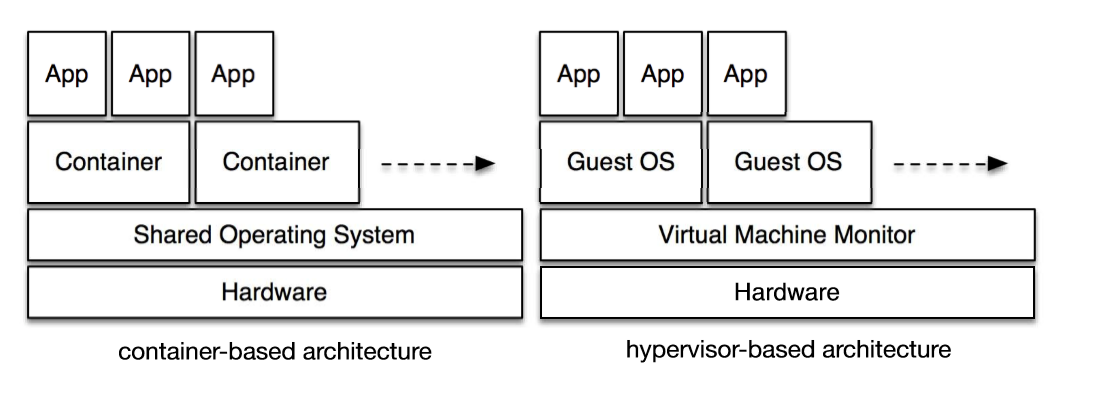
\includegraphics[width=1\linewidth]{pics/docker2.png}
	\captionof{figure}[Architektur Container und Virtuelle Maschine]{Architektur Container und Virtuelle Maschine \cite{Xavier2015AClouds}}
	\label{fig:architecture}
\end{minipage}

\subsubsection{Namespaces}
Dank der Einführung von Kernel-Namespaces ist es möglich, Ressourcen des Host-Systems wie CPU, Arbeitsspeicher, I/O und Netzwerk voneinander zu isolieren und diese unter bestimmten Voraussetzungen anderen Prozessen zur Verfügung zu stellen. 

Durch Namespaces werden die Ressourcen des Host-Systems in verschiedene Instanzen gepackt. Der innerhalb eines Namespaces gestartete Prozessaufruf sieht nur seine eigene Instanz und die unterliegende Baumstruktur seiner Kindprozesse. Der Prozess selbst hat die Illusion der vollständigen Ressourcenkontrolle über das komplette System, wobei diesem nur ein zugewiesener Teil zur Verfügung steht.

Aktuell existieren sieben verschiedene Namespaces. Diese sind \ac{PID}-Namespaces, Mount-Namespaces, \ac{UTS}-Namespaces, \ac{IPC}-Namespaces, Network-Namespaces, User-Namespaces und \ac{Cgroup}-Namespaces, die im Folgenden genauer erklärt werden.



\vspace{1em}
\begin{minipage}{\linewidth}
	\centering
	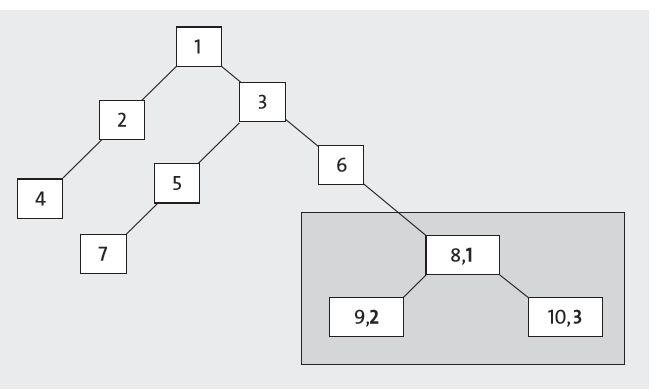
\includegraphics[width=1\linewidth]{pics/PID.PNG}
	\captionof{figure}[PID-Namespaces für Host und Container]{ PID-Namespaces für Host und Container (im Fettdruck) \cite{Liebel2017SkalierbareContainer-Infrastrukturen}}
	\label{fig:PID}
\end{minipage}

\subparagraph{PID-Namespaces} PID-Namespaces sind hierarchisch, deshalb kann ein Prozess nur die anderen Prozesse in seinem eigenen Namespace oder in seinen untergeordneten Namespaces sehen. Folglich kann der Host die Prozesse innerhalb des neuen PID-Namespace des Containers beobachten und beeinflussen. Die Prozesse innerhalb des Containers können die anderen Prozesse, die im Host oder in anderen Containern laufen, nicht beobachten oder beeinflussen. Die vereinfachte Darstellung des PID-Namespaces einer \emph{gespawnten} bzw. \emph{geforkten} Container-Prozess-Umgebung ist in Abbildung \ref{fig:PID} dargestellt. \cite{Liebel2017SkalierbareContainer-Infrastrukturen}

\subparagraph{Mount-Namespaces} Mount-Namespaces isolieren Filesystem Mountpunkte, die von einem Container gesehen werden. Somit können Prozesse in verschiedenen Containern unterschiedliche Ansichten der Filesystemhierarchie haben.

\subparagraph{UTS-Namespaces} UTS-Namespaces erlauben jedem Container seinen eigenen Hostnamen und \ac{NIS}-Domänennamen zu haben.

\subparagraph{IPC-Namespaces} IPC-Namespaces isolieren die Interprozesskommunikation. Das bedeutet, Prozesse die in einem Container enthalten sind, haben eigene Nachrichtenwarteschlangen und sind völlig unabhängig von Prozessen in anderen Containern.

\subparagraph{Network-Namespaces} Network-Namespaces isolieren das Netzwerk-Untersystem wie z.B. Geräte und IP-Adressen. Jeder Container unterhält seine eigene Netzwerkkonfiguration und die darauf laufenden Anwendungen.

\subparagraph{User-Namespaces} User-Namespaces isolieren Benutzer-IDs vom Host und anderen laufenden Containern. Das bedeutet, dass der Benutzer \emph{Root} (ID0) innerhalb eines Containers volle Privilegien hat, außerhalb jedoch keine Privilegien besitzt. Dies gewährleistet vor allem Sicherheit und Zuverlässigkeit \cite{Xavier2015AClouds}.

\subparagraph{Cgroup-Namespaces} Cgroup-Namespaces isolieren Cgroups untereinander, sodass keine Informationen über vorhandene Systemressourcen geteilt werden können.



\subsubsection{Cgroup}
\emph{Cgroup} steht für \ac{Cgroup}. Durch Cgroups ist es möglich, eine Reihe von Kriterien anzuwenden, um Ressourcen wie Speicher, Netzwerk, I/O und CPU einzuschränken. Ein Container sollte seine auferlegten Beschränkungen nicht überschreiten und andere Container, die auf derselben Hardware laufen, nicht stören. Cgroups sind für die Ressourcenbegrenzung, Priorisierung, Abrechnung und Kontrolle zuständig.

Durch Cgroups gibt es einen Weg, um Prozesse und Systemressourcen in einer kontrollierten und konfigurierbaren Weise hierarchisch zu organisieren. Cgroups bestehen im Wesentlichen aus zwei Teilen, dem Kern und dem Controller. Der Cgroup-Kern ist in erster Linie für die hierarchische Organisation von Prozessen zuständig. Der Cgroup-Controller ist in der Regel für die Verteilung einer bestimmten Art von Systemressource entlang der Hierarchie verantwortlich. Cgroups bilden eine Baumstruktur. Jeder Prozess im System gehört genau zu einer Cgroup. Alle Unterprozesse (Kindprozesse) eines Prozesses (Elternprozess) gehören zur gleichen Cgroup \cite{Heo2015ControlV2}. 


\paragraph{Ressourcenverteilungs-Modelle}
Cgroup-Controller verfügen über verschiedene Ressourcenverteilungs-Modelle. Diese Modelle sind auf die Art und den Verwendungszweck der Ressource zugeschnitten. Der folgende Paragraph befasst sich mit den verschiedenen Hauptschemen und deren Aufgaben \cite{Heo2015ControlV2}.

\subparagraph{Weight}
Beim Weight-Modell werden die zur Verfügung stehenden Ressourcen eines Prozesses proportional zur Gewichtung an alle aktiven Kindprozesse verteilt. Da nur die aktiven Kindprozesse, welche aktuell Ressourcen benötigen, an der Verteilung teilnehmen, sind die zugeteilten Ressourcen effizient genutzt. 

\subparagraph{Limit}
Das Limit-Modell bietet die Möglichkeit, verschieden Limits zu verwenden. Ist ein High-Limit gesetzt, kann ein Kindprozess die Ressource nur bis zu der konfigurierten Menge verwenden. Low/High-Limits können auch als Soft-Limits bezeichnet werden. Die Summe der Limits aller Kindprozesse kann die zur Verfügung stehende Menge an Ressourcen des Elternprozesses überschreiten. Ein Limit ist sozusagen ein maximaler Richtwert, der bei dringendem Bedarf überschritten werden kann. Der Prozess, welcher den über das Limit hinausragenden Anteil verwendet, steht unter erhöhtem Druck und wird gedrängt, die Ressource schnell wieder frei zu geben. Wenn eine Cgroup die Ressourcen nicht mehr benötigt, wird diese bis zu einem setzbaren Low-Limit freigegeben.


\subparagraph{Protection}
Im Protection-Modell ist eine Cgroup so geschützt, dass sie bis zur konfigurierten Menge der Ressource fest zugeordnet werden kann, solange die Verwendung aller Prozesse unter der geschützten Ebene liegt. Der Schutz kann garantiert oder effizient sein. Bei garantiertem Schutz wird die Ressource explizit für die Cgroup freigehalten und kann vollständig verwendet werden. Die effizientere Variante bietet die Möglichkeit, zugeteilte Ressourcen auf Anfrage für andere Prozesse freizustellen.


\subparagraph{Allocation}
Einer Cgroup wird eine bestimmte Menge einer Ressource fest zugeteilt und stellt somit ein Hard-Limit dar. Die Summe der Zuweisungen von Kindprozessen darf die Menge der fest zugeteilten Ressourcen des Elternprozesses nicht überschreiten. Auch wenn die Ressource nicht vollständig ausgenutzt wird, bleibt diese der Cgroup erhalten. 


\paragraph{Ressourcen-Modellierung}
Da nicht jede Hardwareressource auf die gleiche Art eingeschränkt werden kann, existieren Controller, die anhand der gerade beschriebenen Modelle, Ressourcen verwalten. Im folgenden Paragraphen werden die Art der Ressource mit den verwendeten Modellen genauer betrachtet, sowie unterschiedliche Varianten der Limitierung aufgezeigt. Besonderes Augenmerk ist auf die Speicherverwaltung gelegt.

\subparagraph{Speicher}
Der Speicher-Controller regelt die Verteilung des Speichers. Speicher ist zustandsabhängig und verwendet sowohl Limit- als auch Protection-Modelle. Aufgrund der Verflechtung zwischen Speicherbedarf und Speicherrückgabeforderung ist die Verwaltung sehr kompliziert.

\emph{Memory-Low (best-effort)}
Der geforderte Mindestanteil wird gestellt. Unbenutzter Speicher kann bei Bedarf vom System verwendet werden.

\emph{Memory-High (best-effort)}
Dies ist der Hauptmechanismus zur Steuerung des Speicherverbrauchs einer Cgroup. Wenn die Nutzung einer Cgroup über die obere Grenze hinausgeht, werden die Prozesse der Cgroup gedrosselt und unter starken Reklamationsdruck gesetzt.

\emph{Memory-Min (hard-limit)}
Falls der Speicherverbrauch einer Cgroup innerhalb seiner effektiven minimalen Grenze liegt, wird der Speicher der Cgroup unter keinen Umständen zurückgefordert. Wenn nicht genug Speicherplatz zur Verfügung steht um die Minimalanforderung zu gewährleisten, kommt der OOM-Killer (siehe Kapitel \ref{Isolation Container}) zum Einsatz und schafft freien Speicher.

\emph{Memory-Max (hard-limit)}
Wenn der Speicherverbrauch einer Cgroup diese gesetzte Grenze erreicht und nicht reduziert werden kann, wird der OOM-Killer in der Cgroup aufgerufen. Dies ist der letzte Schutzmechanismus. Unter bestimmten Umständen kann ein Prozess vorübergehend über das Limit hinaus gehen.

\subparagraph{CPU}
Der CPU-Controller reguliert die Verteilung der CPU-Zyklen. Diese Steuerung verwendet Weight- und Limit-Modelle für normale Ressourcenverteilung und das Allocation-Modell für eine Echtzeitverteilung.

\subparagraph{I/O}
Der I/O-Controller reguliert die Verteilung der I/O-Ressourcen. Der Controller verwendet Weight- und Limit-Modelle. Die Gewichtung gibt die relative I/O-Zeit an, welche die Cgroup in Bezug auf ihre Geschwister verwenden kann.

\subsection{Hypervisor-basierte Virtualisierung}
Eine \ac{VM} bildet mit Hilfe des \emph{Hypervisors}, auch \ac{VMM} genannt, eine komplette Rechnerarchitektur auf dem Host-Rechner ab (siehe Abbildung \ref{fig:architecture}). Der Hypervisor ist ein modifizierter minimaler Betriebssystem-Kernel. Man unterscheidet zwischen zwei Arten von VMM: Dem Typ-1-VMM oder \emph{bare-metal-hypervisor}, welcher direkt auf der zugrundeliegenden Hardware des Hosts liegt und dem Typ-2-VMM \emph{hostet-hypervisor}, der eine komplette virtuelle Maschine auf dem Host-Betriebssystem erstellt. Die Grundanforderung eines VMM sind nach Popek/Goldberg \cite{Popek1974FormalArchitectures,Glatz2015Betriebssysteme}:


 \subparagraph{Equivalence} 
 Prozesse, die auf der virtuellen Maschine gestartet werden, laufen wie Prozesse auf dem  Host-System identisch ab, mit Ausnahme der Geschwindigkeit. 
 
\subparagraph{Efficiency} 
Alle unkritischen Prozesse werden von der Hardware direkt ausgeführt, ohne Eingreifen des VMM.

\subparagraph{Resource control} 
Es darf kein Prozess Ressourcen verwalten. Bei jedem Zugriffsversuch eines Prozesses auf Systemressourcen wird der VMM aufgerufen.



\subsubsection{Typ-1-VMM}
Der bare-metal-hypervisor, schematisch dargestellt in Abbildung \ref{fig:Hypervisor_Typ1/Typ2} a, liegt direkt auf der Hardware und hat uneingeschränkten Zugriff darauf. Der VMM kümmert sich um die Ressourcenverwaltung und die isolierte Bereitstellung von virtuellen Maschinen. Die Aufteilung der Rechenzeit (CPU) und die Zuteilung von Speicher auf die einzelnen VMs sind Beispiele der Aufgaben, welche die Ressourcenverwaltung beinhaltet. Dieser Virtualisierungsansatz wird beispielsweise von \emph{Xen} \cite{Install2018XenArchitecture} verwendet,  der nur mit einem eigenen, auf die Hardware zugeschnittenen Treiber, laufen kann \cite{Glatz2015Betriebssysteme}.

\vspace{1em}
\begin{minipage}{\linewidth}
	\centering
	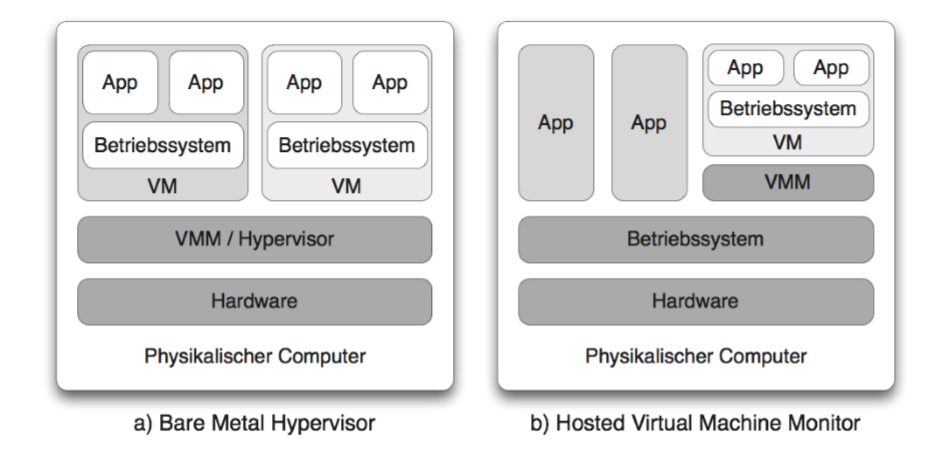
\includegraphics[width=1\linewidth]{pics/Hypervisoren.PNG}
	\captionof{figure}[Hypervisor Typ1/Type2]{Hypervisor Typ1-/Typ-2 \cite{Meinel2011VirtualisierungMarktubersicht} }
	\label{fig:Hypervisor_Typ1/Typ2}
\end{minipage}

\subsubsection{Typ-2-VMM}
Ein gehosteter Hypervisor teilt sich ein Host-Betriebssystem mit anderen Applikationen (siehe Abbildung \ref{fig:Hypervisor_Typ1/Typ2} b). Um die nötigen Rechte auf der Hardware zu erhalten, wird ein spezieller VMM-Treiber verwendet, der direkt unter dem Host-System installiert wird. Dieser ermöglicht privilegierten Zugriff auf die Hardware. \emph{VMware Workstation} ist ein Produkt dieser Realisierung der Virtualisierung \cite{Glatz2015Betriebssysteme}.

\subsubsection{Hybridformen}
Hypervisor die von Haus aus direkt in das Betriebssystem integriert wurden, sind zwischen Typ-1 und Typ-2 anzusiedeln. Die Realisierung von Linux heißt \ac{KVM}, das Pendant von Windows ist \emph{Hyper-V}. Diese Hybridformen sind die aktuell performantesten Hypervisor. 

\subsubsection{Hypervisor Virtualisierungsformen}
 Ressourcenanfragen, die das Gastsystem an die CPU sendet, müssen von der Virtualisierungsschicht (Hypervisor) abgefangen und interpretiert werden \cite{Meinel2011VirtualisierungMarktubersicht}. Das geschieht entweder über vollständige, Para- oder hardwareunterstütze Virtualisierung.  Es gibt bei aktuellen Prozessoren eine Rechteverwaltung, welche als Ringdiagramm darstellbar ist, siehe Abbildung \ref{fig:Ringmodell1}. Im Ring 0 besitzt man volle Zugriffsrechte auf Hardwareressourcen. Auf dieser Ebene ist der Kernel beheimatet. Die Ringe 1 und 2 stehen für Treiber zur Verfügung und in Ring 3, der die eingeschränktesten Zugriffsrechte enthält, sind alle sonstigen Anwendungen beheimatet. Die Kernel der Gastbetriebssysteme befinden sich grundsätzlich ebenfalls in dem 3. Ring. Im Folgenden wird genauer auf die drei eben erwähnten Virtualisierungsmethoden eingegangen. Eine Zusammenstellung der Virtualisierungmethoden ist in Abbildung \ref{fig:Virtualisierungen_Hypervisor} dargestellt.

\subparagraph{Vollständige Virtualisierung}
 Wenn eine Anwendung mit einem \emph{Systemcall} direkt auf einen vom Host-Kernel reservierten Speicherbereich zugreifen will, tritt eine Speicherschutzverletzung auf. Der Zugriff wird verweigert, was den Prozess abstürzen lässt. Der Hypervisor fängt solche kritischen Anfragen ab, überprüft diese, codiert die Anfragenstellung gegebenenfalls um und führt sie selbst mit höheren Zugriffsrechten aus. Nach dem Aufruf folgt eine entsprechende Rückübersetzung und Rückgabe an die aufrufende virtuelle Maschine. Diesen Vorgang nennt man \emph{binary translation}, der sehr häufig durchgeführt werden muss. Dies führt zu einem erheblichen Overhead, der signifikante Leistungseinbußen zur Folge hat \cite{Meinel2011VirtualisierungMarktubersicht}. 
 
 \vspace{1em}
\begin{minipage}{\linewidth}
	\centering
	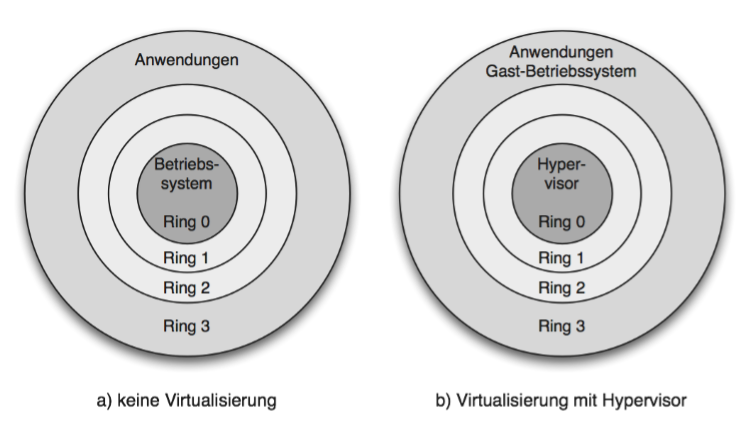
\includegraphics[width=1\linewidth]{pics/Ringmodell1.PNG}
	\captionof{figure}[Ringdiagramm Zugriffsverwaltung ]{Ringdiagramm Zugriffsverwaltung \cite{Meinel2011VirtualisierungMarktubersicht} }
	\label{fig:Ringmodell1}
\end{minipage}
 
 \subparagraph{Para-Virtualisierung}
 Bei der Para-Virtualisierung werden die Kernel der Gastbetriebssysteme so angepasst, dass diese auf Ring 1 laufen können. Was vorher \emph{Systemcalls} waren und vom Betriebssystem verweigert wurden, sind jetzt \emph{Hypercalls}, die direkt an den Hypervisor gesendet werden. Der Hypervisor führt den entsprechenden Systemaufruf aus und bedient die aufrufende virtuelle Maschine \cite{Meinel2011VirtualisierungMarktubersicht}. Um diese effizientere Methode der Virtualisierung zu verwenden, ist eine darauf zugeschnittene Hardware nötig.

\vspace{1em}
\begin{minipage}{\linewidth}
	\centering
	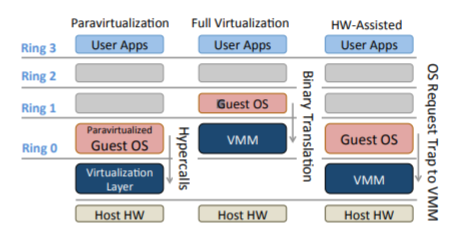
\includegraphics[width=0.8\linewidth]{pics/Virtualisierungen_Hypervisor.PNG}
	\captionof{figure}[Virtualisierungen Hypervisor]{Virtualisierungen Hypervisor \cite{Fayyad-Kazan2013BenchmarkingHypervisors}}
	\label{fig:Virtualisierungen_Hypervisor}
\end{minipage}
 
\subparagraph{Hardwareunterstützte Virtualisierung}
Durch die Hardwareunterstützung von \emph{Intel VT-x} \cite{TechnologyIntel} oder \emph{AMD-v} \cite{AMDVirtualisierungstechnologie}, die den Prozessor-Befehlssatz erweitern, können virtuelle Maschinen \emph{Systemcalls} nativ ausführen. Somit müssen die Kerne der Gastbetriebssysteme nicht modifiziert werden, wie es bei der Para-Virtualisierung gemacht wird. Die hardwareunterstützte Variante ist die performanteste Methode der Hypervisor-Technologien \cite{Meinel2011VirtualisierungMarktubersicht}.




%\pagebreak


% ----------------------------------------------------------------------------------
% Kapitel: Softwarelösungen
% ----------------------------------------------------------------------------------

\thispagestyle{empty}

\section{Softwarelösungen}

\subparagraph{Linux-VServer}
Linux-VServer ist eine der ältesten Implementierungen von Linux-Container-basierten Systemen. Anstatt Namespaces zu verwenden, benutzt Linux-VServer selbst eingeführte Funktionen im Linux-Kernel, um die Isolation zu gewährleisten, wie z.B. Prozessisolation, Netzwerkisolation und CPU-Isolation. Linux-VServer verwendet den traditionellen Aufruf des Chroot-Systems, um das Filesystem innerhalb der Container einzusperren. Auf diese Weise schränkt es den Umfang des Filesystems für die Prozesse ein. Die Prozessisolierung erfolgt durch einen globalen PID-Raum, der alle Prozesse außerhalb des Bereichs eines Containers verbirgt und unerwünschte Verbindungen zwischen Prozessen verschiedener Container verhindert. Das wichtigste Merkmal dieses Ansatzes ist die Skalierbarkeit für eine große Anzahl von Containern. Der Nachteil ist jedoch die Unfähigkeit des Systems, die üblichen Virtualisierungstechniken wie Live-Migration, Checkpoint und Wiederherstellung zu implementieren, da es nicht möglich ist, Prozesse mit derselben PID neu zu initiieren. Linux-VServer virtualisiert keine Netzwerk-Subsysteme. Vielmehr werden alle Netzwerk-Subsysteme (wie Routingtabellen und IP-Tabellen) von allen Containern gemeinsam genutzt. Dieser Ansatz setzt einen Identifier-Tag um zu vermeiden, dass ein Container Netzwerkverkehr zu anderen Containern empfangen kann. Entsprechende Filter sind im Netzwerkstack hinterlegt, um sicherzustellen, dass nur der richtige Container die Daten empfangen kann. Die Container sind nicht in der Lage, ihre eigenen Routingtabellen- und IP-Tabellen zu ändern, was vom Host-Administrator durchgeführt werden muss. 

Um die CPU-Isolation zu gewährleisten, verwendet Linux-V Server den Standard-Linux-Scheduler, der durch das \emph{Token Bucket Filter} (TBF)-Schema überlagert wird. Jedem Container ist ein Token Bucket zugeordnet, der dazu dient, Token mit einer bestimmten Geschwindigkeit zu sammeln. Auf diese Weise ist jeder Prozess bei der Erstellung eines Token mit einem Container verbunden. Diese Token werden bei der Ausführung auf der CPU im Container Bucket bis zu einer bestimmten Mindest- oder Maximalanzahl gesammelt. Dieses Token Bucket-Schema kann verwendet werden, um eine faire Aufteilung der CPU zu gewährleisten. Ressourcenbegrenzungen wie Speicherverbrauch und Anzahl der Prozesse werden mit Systemaufrufen (\emph{rlimit-Tool}) des Linux-Kernels durchgeführt. Die neuesten Versionen von Linux-VServer bieten jedoch Unterstützung für Cgroup, mit denen auch die CPU-Auslastung und der Speicherverbrauch von Containern eingeschränkt werden können. Die Linux-VServer Container werden vom \emph{util-vserver} \cite{Optionen2018Userspace-WerkzeugeLinux-VServer} Package verwaltet \cite{Overview2018PaperLinux-VServer} \cite{Xavier2015AClouds}.

\subparagraph{OpenVZ}
OpenVZ bietet eine ähnliche Funktionalität wie Linux-VServer. Es basiert jedoch auf Kernel-Namespaces, wodurch es sicherstellt, dass jeder Container seine eigene isolierte Teilmenge einer Ressource erhält. Das System verwendet PID-Namespaces, um die Prozessisolierung zwischen Containern zu gewährleisten. Darüber hinaus ermöglichen PID-Namespaces übliche Virtualisierungstechniken wie Live-Migration, Checkpoint und Widerherstellungsmethoden. In OpenVZ hat dank IPC-Namespaces jeder Container seinen eigenen Semaphoren- und Nachrichtenspeicher. Außerdem werden Network-Namespaces genutzt. OpenVZ verwendet vier Ressourcenmanagementkomponenten: \emph{User Beancounter} (UBS), faires CPU-Scheduling, \emph{Disk Quota} und I/O-Scheduling. UBS bietet die Möglichkeit der Limitierung der Ressourcen, die auf jedem Container kontrolliert werden. Der OpenVZ CPU-Scheduler funktioniert auf zwei Arten, um eine faire Verteilung zu generieren. Zum einen wird entschieden, welcher Container als nächstes auf dem Prozessor ausgeführt werden darf, zum anderen wird anhand einer Prioritätenliste die Reihenfolge der Prozesse des Containers erstellt. Ein weiteres Konzept ist die \emph{VCPU Affinity}, welches die maximale Anzahl an CPUs definiert, die ein Container verwenden darf. \emph{Disk Quota} ist eine Funktion, mit der eine Begrenzung des Speicherplatzes auf einem Speichermedium für einzelne Benutzer oder eine Gruppe von Benutzern festgelegt werden kann. Schließlich wird ein ähnlicher Ansatz des CPU-Scheduling für I/O-Scheduling verwendet. Das Verfahren ist wieder in zwei Teile aufgeteilt. Der erste Teil funktioniert genau wie beim CPU-Scheduling, der zweite Teil wird anhand des \emph{Completely Fair Queuing} (CFQ) Algorithmus festgelegt. Jeder Container besitzt eine I/O-Priorität, der I/O-Scheduler verteilt die verwendbare Bandbreite anhand der Priorisierung. Auf diese Weise kann nicht ein einzelner Container den kompletten Kanal beanspruchen. OpenVZ Container werden durch \emph{vzctl} \cite{ParallelsIPHoldingsGMbH2018Vzctl} verwaltet \cite{IndexOpenvz.org} \cite{Xavier2015AClouds}.

\subparagraph{Linux Container}
Ähnlich wie OpenVZ verwendet LXC Kernel-Namespaces, um die Ressourcenisolierung zwischen allen Containern zu gewährleisten. Während dem Start des Containers werden standardmäßig PIDs, IPCs und Mount Points virtualisiert und über den PID-Namespace, den IPC-Namespace bzw. den Mount-Namespace isoliert. Um mit der Außenwelt zu kommunizieren und die Netzwerkisolierung zu ermöglichen, verwendet LXC die Netzwerk-Namespaces. Im Gegensatz zu Linux-VServer und OpenVZ ist die Ressourcenverwaltung nur über Cgroups erlaubt. Die Prozesskontrolle wird ebenfalls über Cgroups durchgeführt. I/O-Operationen sind wie in OpenVZ ebenfalls durch den CFQ-Scheduler gesteuert \cite{IndexLinuxcontainers.Org} \cite{Xavier2015AClouds}.

\subparagraph {Xen}
Xen ist eine Virtualisierungslösung, die ursprünglich an der \emph{University of Cambridge} entwickelt wurde. Xen ist die einzige Bare-Metall-Lösung, die als Open Source als Grundlage für eine Reihe verschiedener kommerzieller und Open Source Anwendungen dient. Xen besteht aus mehreren Komponenten, die zusammenwirken, um eine Virtualisierungsumgebung bereitzustellen. Die Hauptbestandteile sind Xen-Hypervisor, Domain0 Gast (Dom0) und DomainU Gast (DomU), die entweder Para-virtualisiert, vollständig-virtualisiert oder hardwareunterstützt-virtualisiert sein können. Der Xen-Hypervisor ist eine Softwareschicht, die direkt auf der Hardware unter allen Betriebssystemen läuft. Er ist für das CPU-Scheduling und die Speicherpartitionierung der verschiedenen VMs, die auf der Hardwarevorrichtung laufen zuständig. Wenn Xen startet, übernimmt der Xen-Hypervisor die Kontrolle über das System und lädt das erste Gastbetriebssystem auf Dom0. Dom0 ist ein modifizierter Linux-Kernel, der eine einzigartige Virtuelle Maschine darstellt. Dieser läuft auf dem Xen-Hypervisor mit priveligierten Zugriffsrechten auf physische I/O-Ressourcen und speziellen Rechten für die Interaktion mit anderen Virtuellen Maschinen. Die auf der DomU ausgeführten modifizierten Betriebssysteme besitzen keinen direkten Zugriff auf physische Daten. Seit Xen Version 3.0 ist \emph{CREDIT} der Standard Xen-Scheduler, um die CPU fair auf die Virtuellen Maschinen aufzuteilen. Im Credit-Scheduler wird jeder VM eine Gewichtung zugewiesen, anhand derer die CPU-Ressourcen auf die Systeme verteilt werden \cite{Fayyad-Kazan2013BenchmarkingHypervisors}. 

\subparagraph {VMware Workstation}
VMware Workstation wurde 1998 entwickelt um die x86 Architektur zu virtualisieren ohne Hardware oder Software zu ändern. Infolgedessen unterscheidet sich VMware Workstation von den klassischen Überwachungen Vitueller Maschinen. Um die Virtualisierung in bestehende Systeme einzubinden, kombiniert VMware Workstation eine gehostete Architektur mit einem \emph{Virtual Machine Monitor} (VMM). Die gehostete Architektur ermöglicht eine einfache Benutzerführung und bietet eine breite Hardwarekompatibilität. Die Architektur ermöglicht es, bei minimaler Beeinträchtigung den gemeinsamen Vorsitz auf Systemebene zwischen einem Host-Betriebssystem und einem VMM zu übernehmen. Anstatt die I/O-Diversität der x86-Plattform den Virtuellen Maschinen auszusetzen, setzt VMware Workstation auf die SoftwareEmulation von kanonisch ausgewählten I/O-Geräten und ermöglicht damit auch die hardwareunabhängige Kapselung von Virtuellen Maschinen. Der VMWare VMM kompensiert den Mangel an architektonischer Unterstützung für die Virtualisierung durch die Kombination einer Direct Execution Engine mit einem Binärübersetzer auf Systemebene, um die x86-Architektur effizient zu virtualisieren und die meisten gängigen Betriebssysteme zu unterstützen. Der VMM verwendet die Segmentierung als Schutzmechanismus, sodass sein binär übersetzter Code mit nahezu Hardware-Geschwindigkeiten ausgeführt werden kann. Der VMM bietet auch adaptive binäre Übersetzung, um den Overhead der Virtualisierung von Speicher stark zu reduzieren \cite{Bugnion2012BringingWorkstation}.


\subparagraph{KVM}
\emph{Kernel Virtual Machine} (KVM) ist eine Funktion von Linux, die es ermöglicht, als Typ-1-Hypervisor zu fungieren und ein unmodifiziertes Gastbetriebssystem in einem Linux Prozess zu erstellen. KVM verwendet Hardware-Virtualisierung in aktuellen Prozessoren, um die Komplexität und den Overhead zu reduzieren. Bei Intel \emph{VT-x} oder \emph{AMD-v} erübrigt sich die Notwendigkeit einer komplexen Ring-Rechteverwaltung, welches von früheren Hypervisoren wie Xen und VMware verwendet wurde. KVM verwendet sowohl über \emph{QEMU} \cite{QEMUEmulator} emulierte, als auch via \emph{virtio} \cite{View2018VirtioVirtio} paravirtualisierte I/O-Geräte. Die Kombination aus Hardwarebeschleunigung und paravirtuellem I/O ist entwickelt worden, um den Virtualisierungs-Overhead auf sehr niedrige Werte zu reduzieren. KVM unterstützt die Live-Migration und ermöglicht dadurch die Wartung von physischen Servern oder sogar ganzen Rechenzentren, ohne dass ein Gastbetriebssystem unterbrochen wird. Da eine VM eine statische Anzahl von virtuellen CPUs (vCPUs) und eine feste Menge an Arbeitsspeicher hat, ist der Ressourcenverbrauch natürlich begrenzt. Eine vCPU stellt einen echten CPU-Wert der Zyklen dar und jede Memory-Page des virtuellen Arbeitsspeichers stellt genau eine Memory-Page des realen Rechners dar. KVM kann die Größe von VMs während des Betriebs durch \emph{Hotplugging} und \emph{Ballooning} durch die dafür benötigte Betriebssystemunterstützung verändern. Da jede VM ein Prozess ist, gelten alle normalen Linux-Ressourcenverwaltungsfunktionen in den Virtuellen Maschinen. Das vereinfacht zwar die Implementierung und Verwaltung des Hypervisor, erschwert aber die Ressourcenverwaltung innerhalb des Gastbetriebssystems. Betriebssysteme gehen im Allgemeinen davon aus, dass CPUs immer laufen und der Speicher eine relativ feste Zugriffszeit hat. Unter KVM können vCPUs jedoch ohne Benachrichtigung ausgeplant werden, was zu Performance-Anomalien führt, die schwer zu debuggen sind. Viele Cloud-Anbieter beseitigen diese Probleme, indem sie keine übermäßigen Ressourcen binden, jede vCPU an eine physische CPU koppeln und den gesamten virtuellen Arbeitsspeicher auf den realen Speicher zuschneiden. Dadurch entfällt im Wesentlichen die Planung im Hypervisor. VMs bieten ein gewisses Maß an Isolierung und Sicherheit durch ihre schmale Schnittstelle. Der einzige Weg, über die eine VM mit der Außenwelt kommunizieren kann, ist über eine begrenzte Anzahl von \emph{Hypercalls} oder emulierten Geräten, die beide vom Hypervisor gesteuert werden. Doch auch das ist keine perfekte Lösung. Es wurden Hypervisor-Privilegien-Eskalationsschwachstellen entdeckt, die es einem Gastbetriebssystem ermöglichen, aus seiner VM-\emph{Sandbox} auszubrechen \cite{Felter2014IBMContainers}.

\subparagraph{Hyper-V}
Microsoft Hyper-V ist ein in Windows integrierter Hypervisor, der die Möglichkeit für Para-Virtualisierung und hardwareunterstütze-Virtualisierung bereitstellt. Hyper-V gibt es zudem als eigenständige Version namens \emph{Hyper-VServer} und als installierbares Produkt \emph{Windows Server} Es gibt keine Unterschiede in der Funktionsweise zwischen dem Microsoft Hyper-V. Der Hypervisor ist derselbe, unabhängig von der installierten Variante. MS Hyper-V implementiert die Isolierung von virtuellen Maschinen in Form von Partitionen. Hyper-V unterstütz Para-Virtualisierung und hardwareunterstützte-Virtualisierung. Genau wie bei KVM kann der Performance Overhead reduziert werden. Die Architektur des Hyper-V funktioniert anhand von \emph{micro-kernelized} Hypervisoren. Bei dieser Architektur wird ein Parent/Child System verwendet, wobei die Parent-Partition das Management von Hardwaregeräten organisiert. Das original erstellte Windows Betriebssystem stellt die Parent Partition dar, alle weiteren neu erstellten Virtuellen Maschinen bilden die sogenannten Child-Partitionen. Jeder Zugriff auf virtuelle Geräte wird vom VMBus dirigiert. VMBus ist ein logischer Chanel, welcher die inter-Partitions-Kommunikation verhindert und nur mit berechtigten Partitionen interagiert. Auch der durch Hyper-V zur Verfügung gestellt Hypervisor konnte von einem Benutzer durchbrochen werden. Der Benutzer ist aus der \emph{Sandbox} des Gastbetriebssystems entkommen und hat privilegierten Zugriff auf Ressourcen erhalten \cite{Fayyad-Kazan2013BenchmarkingHypervisors}.



% ----------------------------------------------------------------------------------
% Kapitel: Isolation
% ----------------------------------------------------------------------------------

\thispagestyle{empty}
\section{Isolation}
Dank der Erkenntnisse im Praktischen Abschnitt kann in dieser Section auf den Isolations unterschied der Virtualisierungsmethoden eingegangen werden.

\subsection{Container}
In dieser Arbeit wird ausschließlich Linux verwendet, weshalb auf die Eigenschaften im Linux Kernel eingegangen wird. In einem anderen Betriebssystem können einzelne Punkte unterschiedlich implementiert sein. Die Speicher Verwaltung von Containen übernimmt das darunter liegende Betriebssystem. Weil viele Anwendung Speicher anfragen, bevor sie Ihn verwenden, wurde der Linux kernel mit einer "Over commit" Lösung ausgestattet um Ressourcen effizient zu nutzen. Over commit bedeutet einfach übersetzt Überschulden. Mit dieser Methode wird speicher virtualisiert indem Ressourcen anfragen von Anwendungen vom Kernel immer akzeptiert werden. Dadurch vergibt der Kernel mehr Speicher als auf der Hardware tatsächlich vorhanden ist. Die Anwendungen selbst bekommen genau so viele Memory Pages auf der Hardware, wie sie Aktuell benötigen. Mit diesem System kann es vorkommen, dass mehr Ressourcen benötigt werden als Real vorhanden sind. 

Wenn die Ressourcen auf der Hardware knapp werden, ist Paging die erste Reaktion des Betriebssystems. Beim Paging werden Allokierte aber aktuell nicht verwendete Memory Pages vom Arbeitsspeicher auf den Massenspeicher geladen. Da ein Massenspeicher zugriff sehr aufwändig und langsam ist, wurde diese Möglichkeit der zusätzlichen Speicher Gewinnung limitiert. Auf dem im Praxis Teil verwendeten System liegt das Limit bei 2GB. Wenn Paging nicht ausreicht, wird der "OOM-Killer" aufgerufen. Der Out of Memory-Killer beendet anhand einer Prioritätenliste die niederwertigsten Prozesse, bis ausreichend Platz geschaffen wurde. Jeder Prozess erhält bereits bei der Erstellung eine Priorisierung in Form einer Zahl, die nach Eigenschaft und Wichtigkeit die Priorität wiederspiegelt.

Bei der Erstellung von Containern wird ein in der Maximalen Größe definierter durch C-Group beschränkter und durch Namespace Isolierter Bereich geschaffen. Die aktuelle Größe des Bereichs hängt von den aktuell verwendeten Ressourcen ab und liegt im Regelfall weit unter der maximalen Begrenzung. Mehrere voneinander gut isolierte Container teilen sich ein durch das Betriebssystem verwaltetes Hardwaresystem. Wegen der Speicherverwaltung des Betriebssystems also des Linux Kernels, ist es wie im Praxis teil gezeigt möglich, dass ein Container durch einen erhöhten Speicherverbrauch oder durch eine schlechte Kalkulation des Administrators, mit Hilfe des OOM-Killers Einfluss auf einen anderen Container nehmen kann, was die Illusion der Vollständigen Isolation der Container zerstört.



\subsection{Virtuelle Maschine}
Das Ziel der Prozessisolation ist es, zu verhindern, dass Container untereinander beeinflussbar sind. Dieses Unterfangen ist mit Hilfe der sogenannten "namespaces" möglich. Die Ressourcen Isolation gewährleistet, dass Prozesse nur einen zugeteiltet anteil einer verfügbaren Ressource verwenden können, dies gelingt mit Hilfe der Cgroups.


vllt noch zu erklären!?
Virtuallisierungen
Vollstendige virtuallisierung 
Paravirtualisierung

Hyper-V
KVM

OOM Killer für Fazit


\subsubsection{Sicherheit-Container / Umschreiben!}
In den letzten Jahren unterlag die Entwicklung von Container-Systemen wie Docker, Rocket und andern einer sehr schnellen Evolution. Dabei war der Fortschritt der Technologie wichtiger als die Sicherheit hinter dem System. Es existieren zahlreiche Studien, die alle auf den Schluss kommen, dass viel Potential in der Entwickelten Technologie steckt, doch die Sicherheit noch nicht ausreichend gegeben ist.

Zwei Punkte spielen eine große Rolle. Zum einen die Sicherheit und Vertrauenswürdigkeit der Images, die den Container-Instanzen zugrunde liegen, zum anderen die oben benannten Namespaces. Die Nutzung von Namespaces stellt einen direkten Zugriff auf den Host-Kernel dar, ein Bereich zu dem sich Angreifer bei anderen Systemen erst einmal mühevoll durchkämpfen müssen.


% ----------------------------------------------------------------------------------
% Kapitel: Praktische Umsetzung
% ----------------------------------------------------------------------------------

\thispagestyle{empty}
\section{Praktische Durchführung}
\subsection{Hardware und Software}


\pagebreak
\subsection{Docker}
Die Docker Container Technologie wurde 2013 als das Open Source Projekt \emph{Docker Engine} eingeführt. Basierend auf Linux Container Konzepten nutz auch Docker Namespaces und C-groups zur Isolierung und Limitierung von Containern.  

\subparagraph{Docker Engine}
Docker ist eine client-server Applikation. Der Docker Client kommuniziert mit dem Docker Server oder auch Docker Deamon genannt, der den Großteil der Arbeit übernimmt. Manchmal wird der Docker Deamon auch Docker Engine genannt. Es ist möglich den Docker Deamon und den Docker Client auf demselben Host laufen zu lassen, oder den lokalen Docker Client mit dem Docker Deamon auf einem anderen Host zu verbinden. Die Docker Architektur ist in Abbildung \ref{fig:Docker_Server_Client.PNG} zu sehen\cite{Turnbull2015TheBook}.

\vspace{1em}
\begin{minipage}{\linewidth}
	\centering
	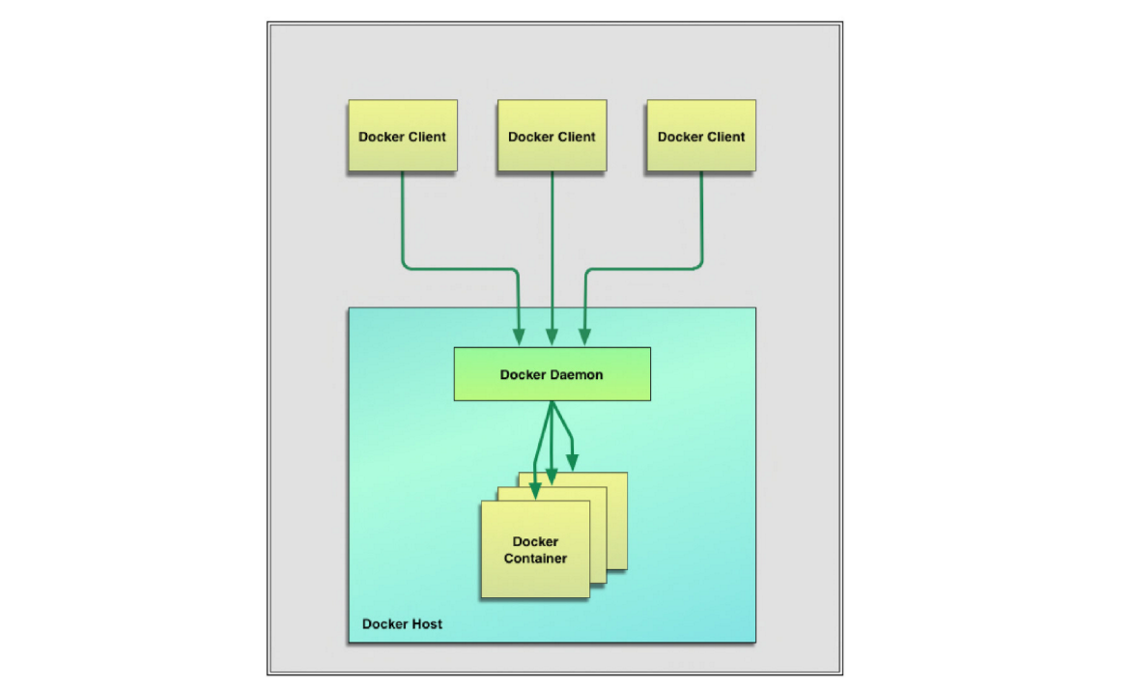
\includegraphics[width=1\linewidth]{pics/Docker_Server_Client.PNG}
	\captionof{figure}[Docker Architektur\cite{Turnbull2015TheBook}]{Docker Architektur}
	\label{fig:Docker_Server_Client.PNG}
\end{minipage}


\subparagraph{Docker Images}
Images sind die Bausteine der Docker Welt. Container werden von Images gestartet. Images sind ein mehrschichtiges Format, die unter Verwendung von Union-Dateisystemen Schritt für Schritt anhand unterschiedlicher Instruktionen erstellt werden. Diese Instruktionen können als Quellcode der Container betrachtet werden. Sie sind einfach verschiebbar und können in Registern verwaltet werden.

\subparagraph{Registries}
Docker speichert die erstellten Images in \emph{Registries}. Es gibt zwei Arten von \emph{Registries}: Öffentliche und private. Docker verwaltet die öffentlichen Images im Docker Hub\cite{DockerInc.2016DockerHub}. Auf Docker Hub können eigene Images abgespeichert und geteilt werden. Diese Plattform beinhaltet bereits Zehntausende Images die von anderen Leuten erstellt wurden, die für eigene Verwendungen zur Verfügung stehen. Private Images kann man ebenfalls auf Docker Hub abspeichern und niemand außer einem ausgewählten Personenkreis hat Zugriff darauf.

\subparagraph{Docker Containers}
Docker unterstützt beim Erstellen und ausführen von Containern. Container werden von Images ausgeführt und können einen oder mehrere Prozesse beinhalten. Images können als der Aufbau Prozess von Docker gesehen werden und Container als die ausführende Instanz von Docker.

Docker leiht sich das Konzept des Standard Schiff Containers die für den Transport von Waren eingesetzt werden, als ein Modell für Docker Container, mit dem Unterschied, dass Docker Container keine Waren, sondern Software transportiert. Container können in jeglicher Umgebung ausgeführt werden. Ob auf dem Laptop, nach dem Download von Docker Hub auf einem Web Server, einem Datenbank- oder auf einem Applikationsserver die Container werden geladen, wie jeder andere Container auch.

\pagebreak

\subsection{Realisierung}
Das in Kapitel 4 genannte Szenario wird in Teilprobleme zerlegt und schrittweise zusammengefügt. Im Ersten Schritt soll gezeigt werden, wie sich der Ressourcenverbrauch eines Containers erhöht und wo eventuelle grenzen der verwendeten Hardware liegen. Im Linux-File-System ist es möglich über die PID eines vorhandenen Prozesses die Cgroup herauszufinden, zu der ein Prozess gehört. Zur Erinnerung, jede Cgroup ist für die Ressourcen Begrenzung, Priorisierung, Abrechnung und Kontrolle aller Prozesse zuständig die unter ihr erstellt wurden. Unter einem Kontrollregister im Linux-Kernel kann die Summe der verwendeten Ressourcen aller unter einer Cgroup laufenden Prozesse zur Laufzeit ausgelesen werden. Die Idee zur Durchführung ist es, einen neuen Docker-Container zu erstellen. In diesem Ruft ein Programm in Endlosschleife den malloc() Befehl auf. Dieses Programm wurde in \emph{C} erstellt. Mit Hilfe der Cgroup wird der Speicherverbrauch des Containers überwacht.

\subparagraph{Test01}
Auf Docker-Hub wird ein geeignetes Image ausgesucht und für den Test erweitert. Beim ausführen des Image wird ein Docker-Container erstellt. Ressourcen Limits können ebenfalls vor dem Starten des Containers eingestellt werden. Für den ersten Start des sind allerdings noch keine Begrenzungen des Speichers nötig, da es in erster Linie um die Auswirkung des ausgeführten C-Programms auf die Ressourcenverwaltung im Container geht. Der verwendete C-Code den der Prozess ausführt, ist in Listing \ref{01mem} zu sehen. Ein erstelltes Skript verwendet die beim Start erzeugte PID, findet die Cgroup in der der Prozess ausgeführt wird und schreibt die ausgelesenen Messdaten in eine Text-Datei. Die Messdaten wie System-Clock-Time in Nanosekunden und Speicherverbrauch in Bytes werden für die Auswertung verwendet.


\vspace{1em}
\lstinputlisting[caption=Einfacher C-Code, label=01mem, basicstyle=\ttfamily\scriptsize]{code/01mem.txt}

\subparagraph{Erwartungshaltung Test 01}
Unter der Annahme, dass das Skript die Messwerte in ungefähr gleichmäßigen Abständen liefert, wird ein linearer Zusammenhang zwischen Zeit und Speicherverbrauch erwartet. Dazu muss die Speicheralokation in jedem Durchlauf stets eine vergleichbare Zeit in Anspruch nehmen. Wenn nicht mehr genug Speicher im System vorhanden ist, wird der OOM-Killer den Prozess beenden.

\vspace{2em}
\begin{minipage}{\linewidth}
	\centering
	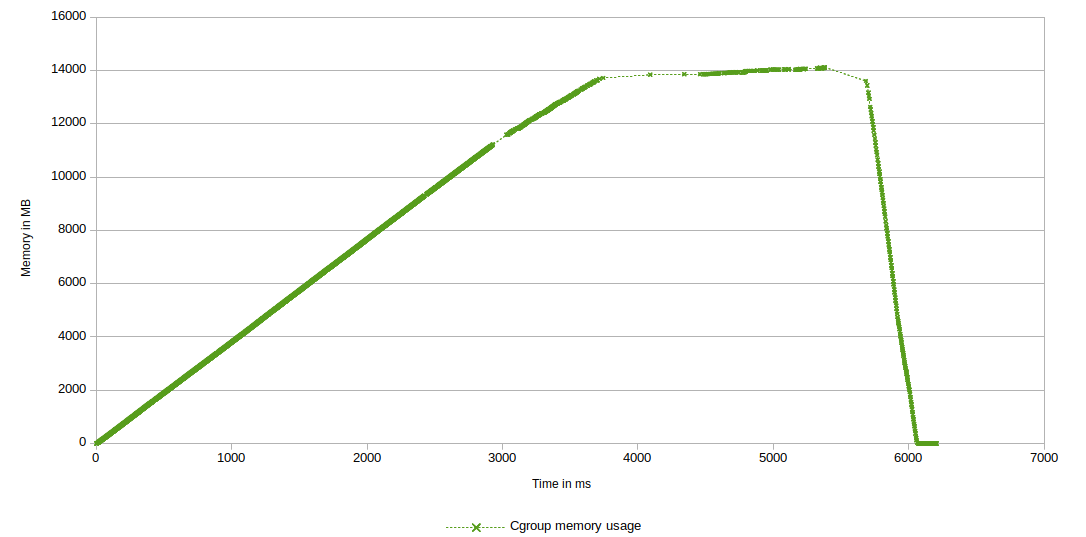
\includegraphics[width=1\linewidth]{pics/001_mem_usage_No_Limit_Cgroup_RDY_FOR_USE.png}
	\captionof{figure}[Speicher Verbrauch Cgroup Ohne Limit]{Memory usage Cgroup no Limit}
	\label{fig:001_mem_usage_No_Limit_Cgroup_RDY_FOR_USE}
\end{minipage}


\subparagraph{Ergebnis Test01}
In Abbildung \ref{fig:001_mem_usage_No_Limit_Cgroup_RDY_FOR_USE} ist wie erwartet ein linearer Zusammenhang erkennbar. Bei ca. 13900MB Allokiertem Speicher sättigt die Kurve. An diesem Punkt ist der insgesamt 16GB große Arbeitsspeicher größtenteils Ausgeschöpft. Ein paar Megabyte konnten vom Betriebssystem für den dauerhaft nach mehr Speicher verlangendem Prozess gefunden werden. Bei knapp über 14000MB wurde der OOM-Killer eingeschaltet um wichtigere Prozesse zu schützen, und der Container wurde beendet.

\subparagraph{Test02}
Im nächsten Schritt wird der Verlauf einer Cgroup näher betrachtet, bei der ein Speicherlimit festlegt wird, das nicht überschritten werden soll (Hard-Limit). Um dieses Limit zu erstellen, wird das Image entsprechend angepasst und das Speicherlimit auf 8200 Megabyte gesetzt. Das in Listing \ref{01mem} vorgestellte Programm wird wieder ausgeführt.

\subparagraph{Erwartungshaltung Test 02}
Da nun ein Hard-Limit eingerichtet ist, Soll die Cgroup mit der gleichen Geschwindigkeit wie in Abbildung \ref{fig:001_mem_usage_No_Limit_Cgroup_RDY_FOR_USE} bis zum gesetzten Limit ansteigt und dieses nicht überschreiten. 

\vspace{1em}
\begin{minipage}{\linewidth}
	\centering
	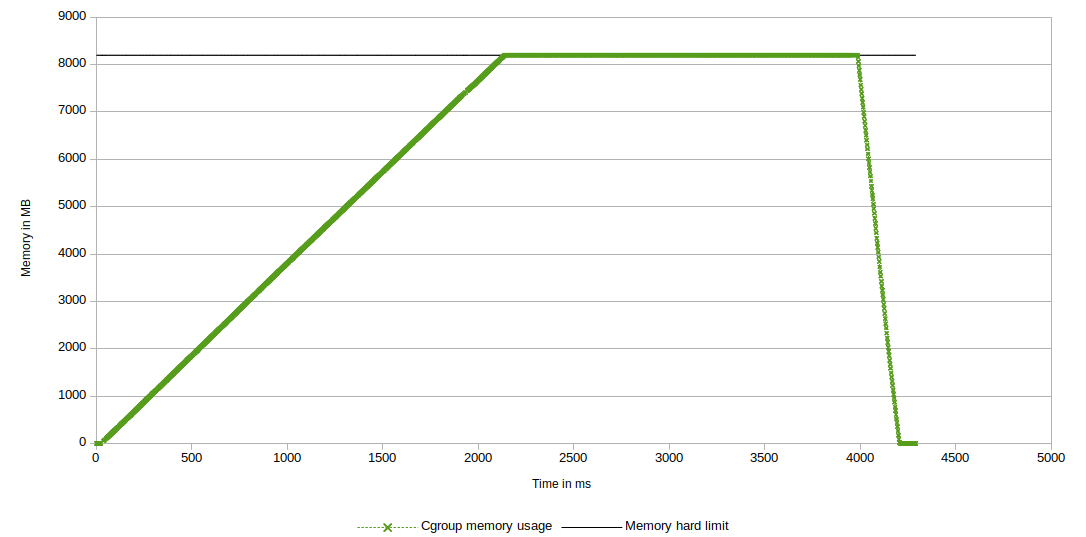
\includegraphics[width=1\linewidth]{pics/002_mem_usage_8200mb_limit_Cgroup_RDY_FOR_USE.png}
	\captionof{figure}[Speicher Verbrauch Cgroup 8200MB Limit]{Memory usage Cgroup 8200MB Limit}
	\label{fig:002_mem_usage_8200mb_limit_Cgroup_RDY_FOR_USE}
\end{minipage}

\subparagraph{Ergebnis Test02}
Mit einer Allokations Rate von ca. 4000MB/S ändert sich die Speicherzugriffsrate nicht. Das Limit von 8200MB wurde erfolgreich eingehalten und der Prozess später vom Betriebssystem beendet.

In Abbildung \ref{fig:001_mem_usage_No_Limit_Cgroup_RDY_FOR_USE}, \ref{fig:002_mem_usage_8200mb_limit_Cgroup_RDY_FOR_USE} tritt eine Sättigung der Speicherallokation ein.  Dies ist aber ohne weiteres nicht zu erklären. Es stellt sich auch die Frage, warum das Programm zu einem Späteren Zeitpunkt vom OOM-Killer beendet wird. Das legt den Schluss nahe, dass das Programm weiterhin Speicher vom Betriebssystem erhält, die Cgroup jedoch nicht in der Lage ist, dies zu erfassen. 

Betrachtet man die Cgroup wie eine Box, ist eine mögliche Erklärung für das oben gezeigte Verhalten herleitbar. Die Größe der Box wird bei der Erstellung des Containers festgelegt. In Abbildung \ref{fig:002_mem_usage_8200mb_limit_Cgroup_RDY_FOR_USE} waren es 8200MB. Der Füllstand der Box setzt sich aus den verwendeten Ressourcen aller in der Box ausgeführten Prozesse zusammen. Wenn ein Prozess wie in Abbildung \ref{fig:002_mem_usage_8200mb_limit_Cgroup_RDY_FOR_USE} die Komplette Box ausfüllt und weiter darüber hinaus ragen würde, wäre die Box nur in der Lage den Füllstand bis zu Ihrer Maximalgröße von 8200 MB widerzuspiegeln. Der Überlaufende Teil des Prozesses kann von der Cgroup nicht erkannt werden.

\subparagraph{Test03}
Nach oben genannten Vermutung liegt es nun nahe, den Speicherverbrauch des Prozesses genauer zu untersuchen. Das Testskript wird erweitert, um die vom Prozess verwendete Anzahl der Memory-Pages auszugeben. Die Anzahl an benötigten Memory-Pages in einem laufenden Prozess, kann ebenfalls im Linux-Kernel ausgelesen werden. Eine Memory-Page ist 4KB groß und ergibt multipliziert mit der verwendeten Anzahl an Memory-Pages die Speichergröße.

\subparagraph{Erwartungshaltung Test 03}
Wenn die Memory-Page Größe multipliziert mit der Anzahl an verwendeten Memory-Pages genau dem entspricht, was die Cgroup an Speicher Allokation ausgibt, sollten beide Graphen bis zum Erreichen des Limits deckungsgleich sein.

\vspace{1em}
\begin{minipage}{\linewidth}
	\centering
	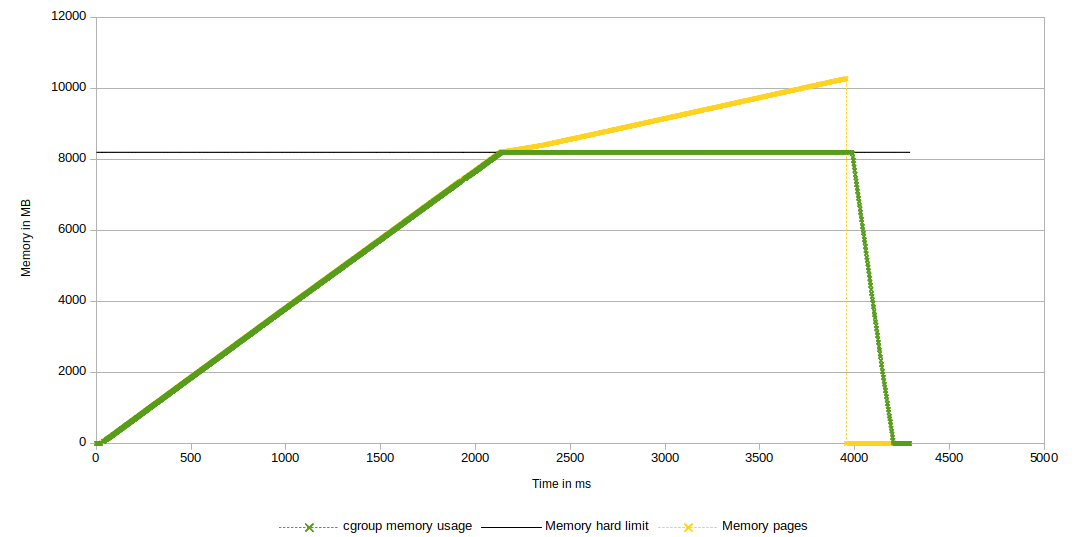
\includegraphics[width=1\linewidth]{pics/003_mem_usage_8200mb_limit_Cgroup_Pages_RDY_FOR_USE.png}
	\captionof{figure}[ Endlosschleife Malloc]{Memory usage Cgroup Memory pages 8200MB Limit Endlosschleife Malloc}
	\label{fig:003_mem_usage_8200mb_limit_Cgroup_Pages_RDY_FOR_USE}
\end{minipage}

\subparagraph{Ergebnis Test03}
Deutlich zu erkennen sind die exakt aufeinanderliegenden Messwerte der Cgroup und der Memory Pages. Ab 8200MB Überschreiten die allokierten Memory Pages bis ca. 10200MB das Limit. Erkennbar ist auch die geringere Allokationsrate die nach dem Überlauf auf 2000MB/s fällt. Komplett ignoriert wurde das Limit allerdings nicht. Verglichen mit Abbildung \ref{fig:001_mem_usage_No_Limit_Cgroup_RDY_FOR_USE} war noch genügend Speicher im System vorhanden. Da stellen sich die Fragen:

Wieso wurde der Prozess dann überhaupt schon beendet, warum konnte er über das Limit hinaus allokieren, wie verhält sich ein Container, wenn er nur ein wenig über das Limit geht, wie wirkt sich das auf andere Container im System aus?

Eine mögliche Antwort ist das sogenannte  \glqq{}\emph{Paging}\grqq{}. Beim Paging werden allokierte aber aktuell nicht verwendete Memory Pages vom Arbeitsspeicher auf den Massenspeicher geladen. In Abbildung \ref{fig:003_mem_usage_8200mb_limit_Cgroup_Pages_RDY_FOR_USE} ist nach 8200MB die Trennung zwischen der Gelben Linie \glqq{}Memory pages\grqq{} und der Grünen Linie \glqq{}Cgroup memory Usage\grqq{} zu erkennen. Zu diesem Zeitpunkt hat das Betriebssystem mit dem Paging begonnen und lädt von dem Prozess allokierte Pages in den Massenspeicher. Die tatsächliche Menge an von der Cgroup allokiertem Arbeitsspeicher auf der Hardware bleibt gleich. Die Gelbe Linie zeigt die Summe aller vom Prozess allokierten Memory Pages, folglich auch den auf den Massenspeicher ausgelagerten Anteil. Die Steigung der Gelben Linie ist einfach nachzuvollziehen. Wegen der Erhöhten Anforderung an das I/O System was das Paging zu verantworten hat, verringert sich die Allokations Rate beim Überschreiten des Limits. Der überlauf von ca. 2GB stimmt mit dem 2GB Paging Limit überein.

\subparagraph{Test03,5}
zur Abklärung und Überprüfung des Paging Limits, empfiehlt sich den Test aus Abbildung \ref{fig:010_mem_usage_8200mb_limit_Container03_undContainer04_RDY_FOR_USE_Focu} mit Erweiterung von Memory Pages zu wiederholen.

\subparagraph{Erwartungshaltung Test03,5}
Es wurden ca. 14000MB beim ersten Testdurchlauf allokiert. Mit dem zusätzlichen Paging Limit von 2GB sind die Memory Pages auf ca. 16000MB zu schätzen. Ein identischer Cgroup Graph wird nicht erwartet, da der Arbeitsspeicherverbrauch des Betriebssystems von mehreren Faktoren abhängt. Doch der Unterschied zwischen Cgroup memory Usage und Memory Pages sollte bei etwa 2GB liegen. 

\vspace{1em}
\begin{minipage}{\linewidth}
	\centering
	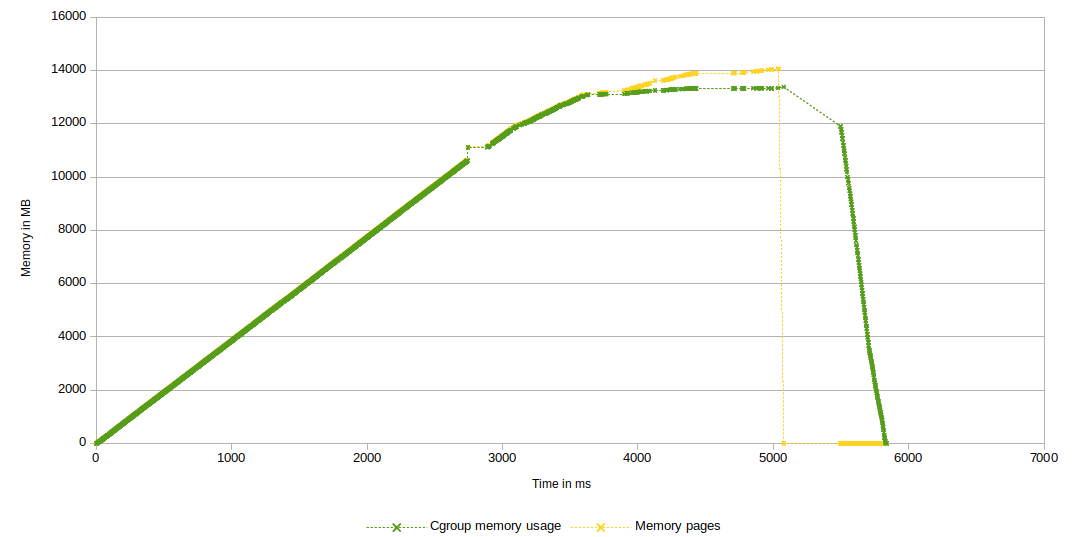
\includegraphics[width=1\linewidth]{pics/001,5_mem_usage_No_Limit_Cgroup_Pages_RDY_FOR_USE.png}
	\captionof{figure}[Speicher Verbrauch Cgroup 8200MB Limit]{Memory usage Cgroup 8200MB Limit}
	\label{fig:001,5_mem_usage_No_Limit_Cgroup_Pages_RDY_FOR_USE.png}
\end{minipage}

\subparagraph{Ergebnis Test03,5}
In Abbildung \ref{fig:001,5_mem_usage_No_Limit_Cgroup_Pages_RDY_FOR_USE.png} sind die 2GB Unterschied zwischen \emph{Cgroup memory usage} und den \emph{Memory Pages} offensichtlich nicht erreicht worden, was mehrere Gründe haben kann. Möglich ist eine zusätzliche Speicheranforderung des Betriebssystems während der Prozess in der Paging Phase war und zum früheren Absturz geführt hat. Auf den Effekt wird im Rahmen dieser Arbeit nicht genauer eingeganen.



\subparagraph{Test04}
Um auf das große Ziel hin zu arbeiten, wird nun ein Container der für eine gewisse Zeitspanne läuft erstellt und etwas mehr als das gesetzte Limit allokiert benötigt. Des in Listing \ref{01mem} gezeigte Programm wird modifiziert und ist in Listing \ref{02mem} zu sehen. 

\vspace{1em}
\lstinputlisting[caption=einfacher C-Code, label=02mem, basicstyle=\ttfamily\scriptsize]{code/02mem.txt}

\subparagraph{Erwartungshaltung Test 04}
Nachdem der Malloc() Befehl jetzt 2200000-mal ausgeführt wird, sollte der Speicherverbrauch der Memory Pages nicht über 8600MB steigen und 60 Sekunden diesen Wert halten.

\[

\mathrm{sizeof(int)} = 4 \mathrm{Byte}

\mathrm{sizeof(int)} * 1024 = 4 \mathrm{KB}

\mathrm{sizeof(int)} * 1024 * 2200000 \approx 8600 \mathrm{MB}\]


\vspace{1em}
\begin{minipage}{\linewidth}
	\centering
	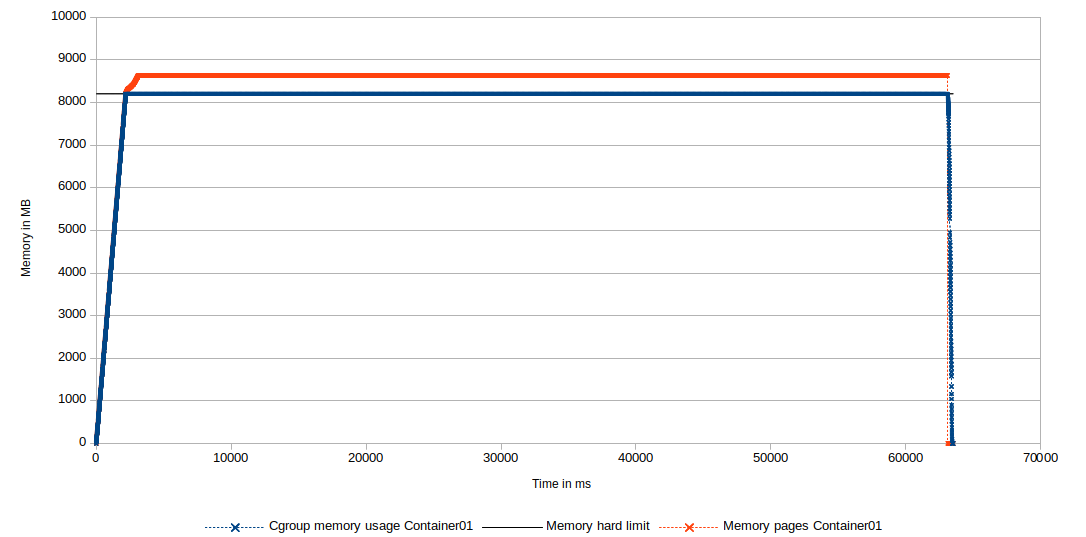
\includegraphics[width=1\linewidth]{pics/004_mem_usage_8200mb_limit_Container01_Basis_RDY_FOR_USE.png}
	\captionof{figure}[Speicher Verbrauch Cgroup 8200MB Limit]{Memory usage Cgroup 8200MB Limit}
	\label{fig:004_mem_usage_8200mb_limit_Container01_Basis_RDY_FOR_USE}
\end{minipage}

\subparagraph{Ergebnis Test04}
Wie in Abbildung \ref{fig:004_mem_usage_8200mb_limit_Container01_Basis_RDY_FOR_USE} zu entnehmen, ist es möglich für einen längeren Zeitraum über das Limit hinaus Ressourcen zu allokieren. Durch die lange Ausführungszeit gleichbleibender Ressourcen ist es jetzt möglich den Einfluss von Container untereinander zu untersuchen. Dieser Container wird von nun an als Container01 bezeichnet.

\subparagraph{Test05}
Im Ablauf des folgenden Tests wird zuerst Container01 gestartet, und während der Laufzeit wird Container02 ebenfalls eingeschaltet. Der Container02 wird zum besseren Verständnis in Abbildung \ref{fig:005_mem_usage_8200mb_limit_Container02_Basis_RDY_FOR_USE_FOCUS} nochmals in skalierter Umgebung dargestellt. 


\vspace{1em}
\begin{minipage}{\linewidth}
	\centering
	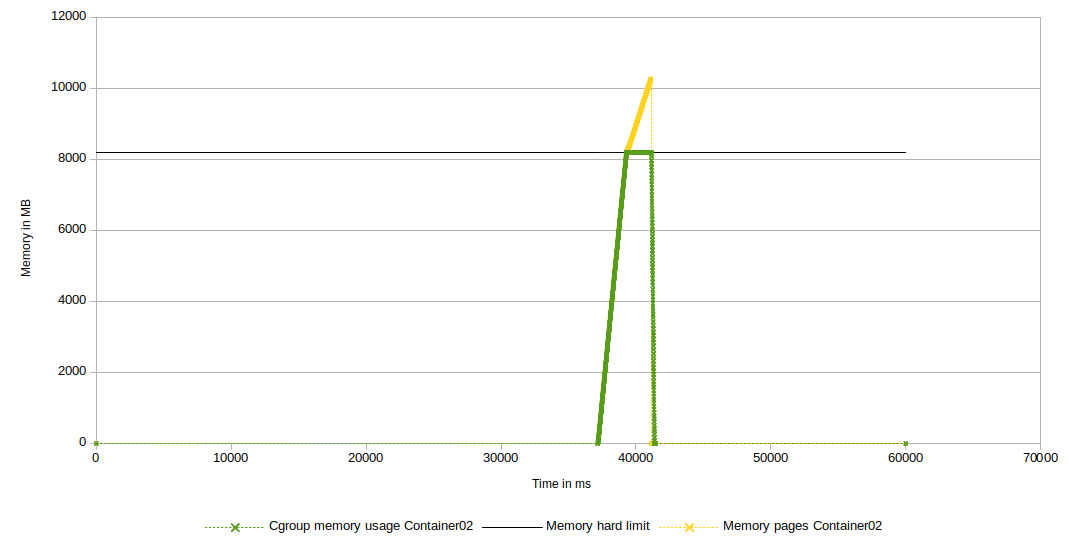
\includegraphics[width=1\linewidth]{pics/005_mem_usage_8200mb_limit_Container02_Basis_RDY_FOR_USE_FOCUS.png}
	\captionof{figure}[Speicher Verbrauch Cgroup 8200MB Limit]{Memory usage Cgroup 8200MB Limit}
	\label{fig:005_mem_usage_8200mb_limit_Container02_Basis_RDY_FOR_USE_FOCUS}
\end{minipage}

\subparagraph{Erwartungshaltung Test 05}
Die verwendbaren Systemressourcen liegen nach Abbildung \ref{fig:001_mem_usage_No_Limit_Cgroup_RDY_FOR_USE} bei etwa 14000MB. Allein Container01 verwendet schon ca. 8600MB der gesamten Summe, was die Deckelung von Container02 auf 8200MB rein rechnerisch unnötig macht. Somit wird Container02 frühzeitig beendet werden. 

\vspace{1em}
\begin{minipage}{\linewidth}
	\centering
	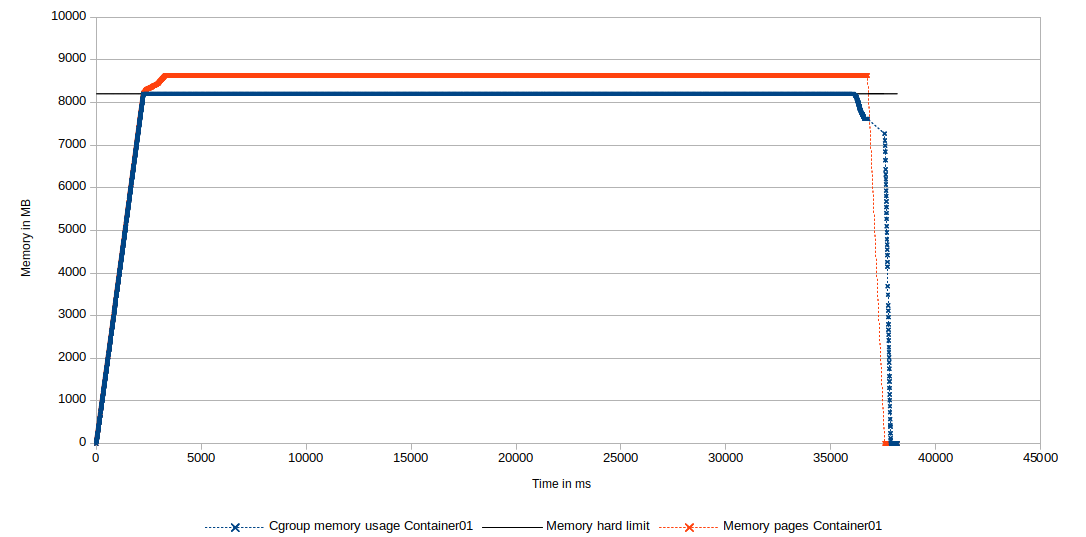
\includegraphics[width=1\linewidth]{pics/006_mem_usage_8200mb_limit_Container01_mit_ipact_RDY_FOR_USE.png}
	\captionof{figure}[Speicher Verbrauch Cgroup 8200MB Limit]{Memory usage Cgroup 8200MB Limit}
	\label{fig:006_mem_usage_8200mb_limit_Container01_mit_ipact_RDY_FOR_USE}
\end{minipage}

\subparagraph{Ergebnis Test05}
In Abbildung \ref{fig:006_mem_usage_8200mb_limit_Container01_mit_ipact_RDY_FOR_USE} ist zu erkennen, dass Container01 nicht nach ca. 63 Sekunden geplant beendet wurde, sondern schon etwa nach ca. 38 Sekunden.

Abbildung \ref{fig:007_mem_usage_8200mb_limit_Container01_und_Container02_RDY_FOR_USE} zeigt beide Container mit einer gemeinsamen Zeitachse. Nach dem Start von Container 02 als dieser ca. 5100MB Speicher Allokiert hat, wird Container 01 beendet. Container 02 überschreitet das Limit von 8200MB nach ca. 41 Sekunden und wird nach ca. 42,5 Sekunden ebenfalls beendet.

\vspace{1em}
\begin{minipage}{\linewidth}
	\centering
	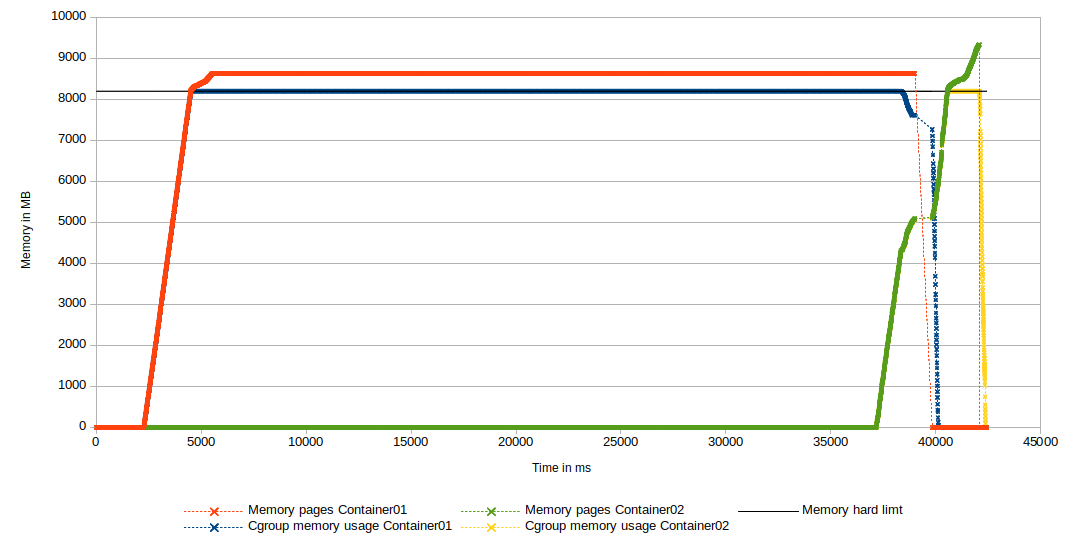
\includegraphics[width=1\linewidth]{pics/007_mem_usage_8200mb_limit_Container01_und_Container02_RDY_FOR_USE.png}
	\captionof{figure}[Speicher Verbrauch Cgroup 8200MB Limit]{Memory usage Cgroup 8200MB Limit}
	\label{fig:007_mem_usage_8200mb_limit_Container01_und_Container02_RDY_FOR_USE}
\end{minipage}

Deutlicher zu sehen ist in Abbildung \ref{fig:008_mem_usage_8200mb_limit_Container01_und_Container02_RDY_FOR_USE_FOCUS} wie die einzelnen Graphen verlaufen. Am auffälligsten ist die große Lücke (mit gestrichelten Linien gekennzeichnet) in der Mitte der Abbildung. Eine Lücke entsteht, wenn über mehrere Millisekunden keine Messwerte vom Skript erfasst werden können. In diesem Fall ist das auf eine Systemüberlastung zurück zu führen, welche durch die Überlastung des Arbeitsspeichers und die dadurch eingeleiteten Systemreaktionen entstanden ist. 

\vspace{1em}
\begin{minipage}{\linewidth}
	\centering
	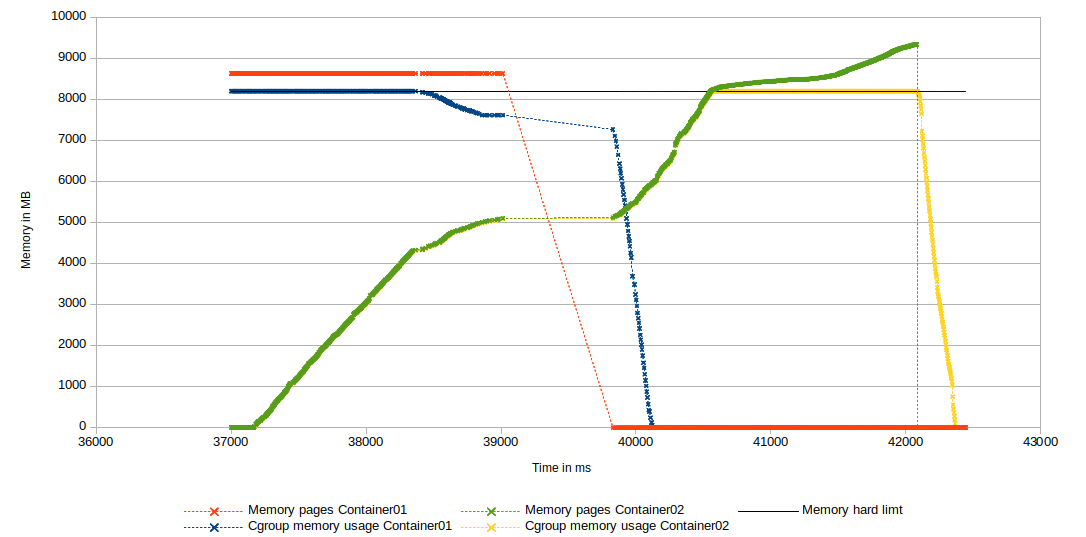
\includegraphics[width=1\linewidth]{pics/008_mem_usage_8200mb_limit_Container01_und_Container02_RDY_FOR_USE_FOCUS.png}
	\captionof{figure}[Speicher Verbrauch Cgroup 8200MB Limit]{Memory usage Cgroup 8200MB Limit}
	\label{fig:008_mem_usage_8200mb_limit_Container01_und_Container02_RDY_FOR_USE_FOCUS}
\end{minipage}



An der blauen Linie \emph{Cgroup memory usage Container01} in Abbildung \ref{fig:008_mem_usage_8200mb_limit_Container01_und_Container02_RDY_FOR_USE_FOCUS} ist nach ca. 38.5 Sekunden ein Abwärtstrend zu erkennen. Zu diesem Zeitpunkt hat das Betriebssystem mit dem Paging begonnen und lädt von der Cgroup allokierte Pages in den Massenspeicher. Die tatsächliche Menge an von der Cgroup allokiertem Arbeitsspeicher wird weniger. Die rote Linie \emph{Memory pages Container01} zeigt die Summe aller vom Prozess allokierten Memory Pages, folglich auch den auf den Massenspeicher ausgelagerten Anteil. Der Verlauf der grünen Linie \emph{Memory pages Container02} lässt sich begründen. Wegen der erhöhten Anforderung an das I/O System was das Paging zu verantworten hat, verringert sich die Allokationsrate. Nach dem Beenden von Container01, was auch das Paging beendet, verläuft die Steigung ähnlich wie nach dem Start des Prozesses. 

\subparagraph{Test06}
Bisher wurden Container betrachtet, die sich nicht an das vorgegebene Limit gehalten haben. Im Folgenden gilt es zu zeigen, dass auch bei \emph{gutartigen} Containern, also Container welche sich immer unter dem vorgegebenen Limit befinden, ähnliche Effekte auftreten. Für den folgenden Testdurchlauf wird der in Listing \ref{03mem} gezeigte C-Code verwendet. Zuerst startet Container03, der den eben genannten C-Code ausführt. Während des 60 Sekunden Sleep() startet Container04 auch mit dem in Container03 verwendeten Code.

\vspace{1em}
\lstinputlisting[caption=einfacher C-Code, label=03mem, basicstyle=\ttfamily\scriptsize]{code/03mem.txt}

\subparagraph{Erwartungshaltung Test 06}
Durch die Änderung auf 2048000 Wiederholungen des Malloc Befehls, wird Container03 bis ca. 8000MB Speicher allokieren. Nach dem Start von Container04 wird ein ähnlicher Graphenverlauf erwartet wie im vorherigen Test. Da das gesetzte Hard Limit bei 8200MB nicht überschritten wird, sollten die Linien \emph{Cgroup memory usage Container04} und \emph{Memory Pages Container04} identisch über die Lebensdauer des Containers verlaufen.

\vspace{1em}
\begin{minipage}{\linewidth}
	\centering
	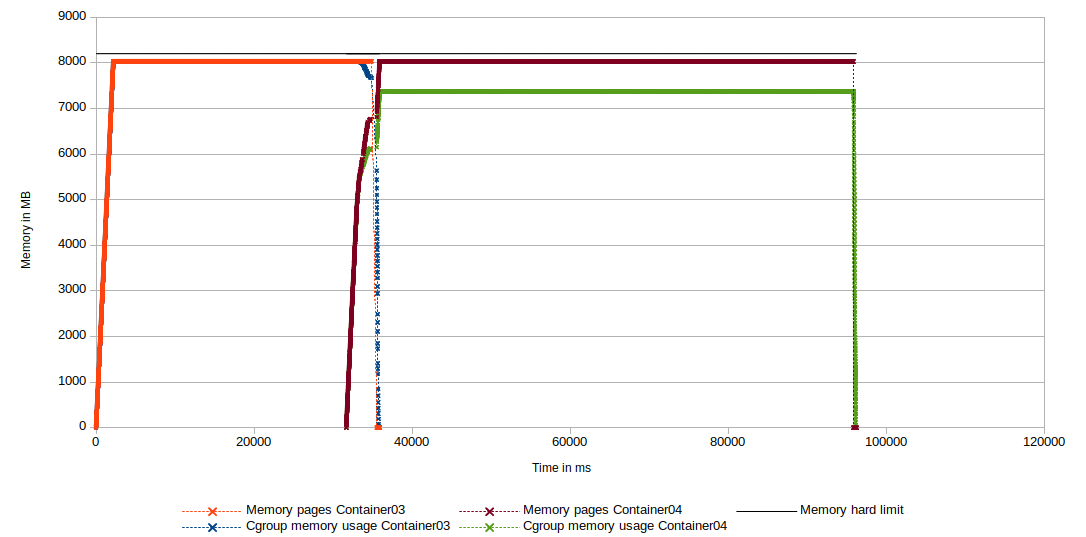
\includegraphics[width=1\linewidth]{pics/009_mem_usage_8200mb_limit_Container03_undContainer04_RDY_FOR_USE.png}
	\captionof{figure}[Speicher Verbrauch Cgroup 8200MB Limit]{Memory usage Cgroup 8200MB Limit}
	\label{fig:009_mem_usage_8200mb_limit_Container03_undContainer04_RDY_FOR_USE}
\end{minipage}

\subparagraph{Ergebnis Test06}
Der Verlauf von Container03 in Abbildung \ref{fig:009_mem_usage_8200mb_limit_Container03_undContainer04_RDY_FOR_USE} war Container01 in Abbildung \ref{fig:007_mem_usage_8200mb_limit_Container01_und_Container02_RDY_FOR_USE} sehr ähnlich. Betrachtet man in Abbildung \ref{fig:010_mem_usage_8200mb_limit_Container03_undContainer04_RDY_FOR_USE_Focu} die Blaue Linie \glqq{}Cgroup memory usage Container03\grqq{} und die dunkelrote Linie \emph{Cgroup memory usage Container04} fällt auf, dass das Betriebssystem nach ca. 33,5 Sekunden mit dem Paging angefangen hat und Einfluss auf die Cgroup beider Container nimmt. Das Resultat ist vergleichbar mit dem aus Abbildung \ref{fig:008_mem_usage_8200mb_limit_Container01_und_Container02_RDY_FOR_USE_FOCUS}.  

\vspace{1em}
\begin{minipage}{\linewidth}
	\centering
	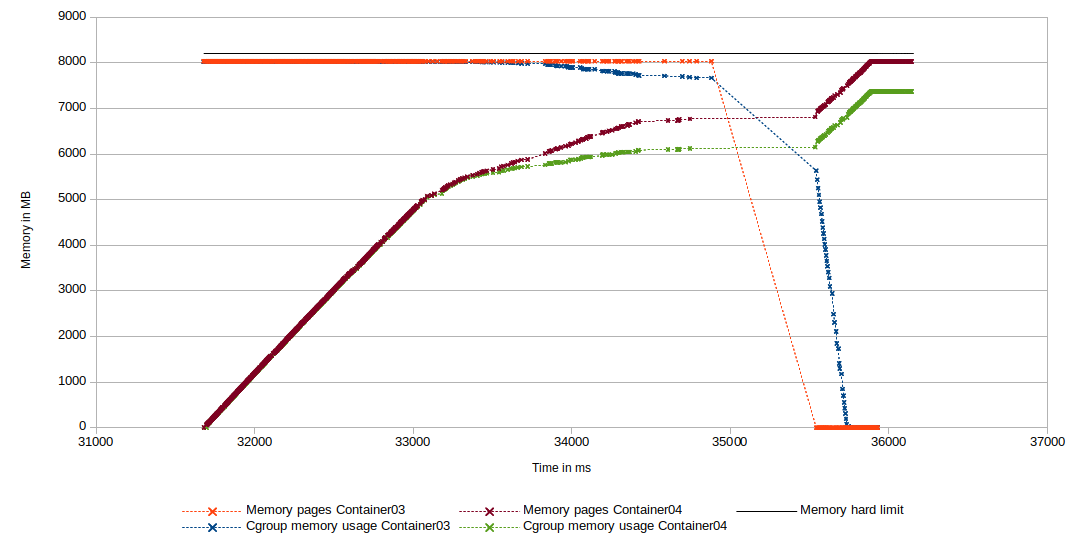
\includegraphics[width=1\linewidth]{pics/010_mem_usage_8200mb_limit_Container03_undContainer04_RDY_FOR_USE_Focus.png}
	\captionof{figure}[Speicher Verbrauch Cgroup 8200MB Limit]{Memory usage Cgroup 8200MB Limit}
	\label{fig:010_mem_usage_8200mb_limit_Container03_undContainer04_RDY_FOR_USE_Focu}
\end{minipage}

Container04 verläuft bei der Allokation unter dem gesetzten Limit wegen des Unterschied von der in Abbildung \ref{fig:009_mem_usage_8200mb_limit_Container03_undContainer04_RDY_FOR_USE} grün dargestellte Linie \emph{Cgroup memory usage Container04} und der dunkelroten Linie \emph{Memory pages Container04} nicht wie erwartet.  In Abbildung\ref{fig:007_mem_usage_8200mb_limit_Container01_und_Container02_RDY_FOR_USE} vor der Lücke war nur die blau dargestellte Linie \emph{Cgroup memory usage Container01} vom Paging betroffen und die Parallel zur grün verlaufende gelbe Linie \emph{Cgroup memory usage Container02} zeigte keine Anzeichen von Paging. Auch an dieser Stelle wird auf den Seiteffekt, verursacht durch das Paging nicht weiter eingegangen.

Es wurde gezeigt, dass ein neu ausgeführter Container mit im Linux-Kernel implementierten Mechanismen in der Lage ist, einen bereits bestehender Container zu beenden und dann auf dessen Ressourcen zuzugreifen.



\pagebreak




% ----------------------------------------------------------------------------------
% Kapitel: Fazit und Ausblick
% ----------------------------------------------------------------------------------

\thispagestyle{empty}
\section{Fazit und Ausblick}


Eine Kette ist nur so stark wie ihr schwächstes Glied. Ob durch einen Hacker angriff oder den Firmeninternen Administrator

Container sind konzipiert um die zur Verfügung gestellte Hardware dynamisch und dadurch effizient zu nutzen. Die Overcommitlösung im Linux-Kernel ist für die Isolation unter den Containern nicht optimal, aber für die Dynamik unerlässlich. Der große unterschied zu einer Hypervisor basierten Virtualisierungsansatz ist genau dieses Overcommitment im Ressourcen-Mangement. Während ein Hypervisor nur die Ihm zur Verfügung stehenden Ressourcen vergibt und nicht die  Ressourcen Selbst virtualisiert, sonder durch die Theoretische Teilung der Hardware mehrere Virtuelle Partitionen erstellt, besteht die Virtuallisierung des Betriebssystem-Kernels aus der Virtuellen Vergrößerung des zur Verfügung stehenden Hardwarebereichs. 

Mit den in dieser Arbeit dargestellten Gefahren von einer zu hohen Auslastung der Ressourcen ist es möglich fallstricke zu umgehen. Mit einer manuellen höheren Prioritätenvergabe im Falle eines OOM-Killer aufrufs von sicheren Containern bei denen die Images und die ausgeführten Programme überprüft wurden, sowie eine Niederwertigen Priorität für unkontrollierte und unwichtigere Container, können zumindest wichtige Prozesse geschützt werden.

Eine Möglichkeit um die Isolation zwischen den Containern zu verstärken und die Prozesse abzusichern, ist die Veränderung des Linux-Kernels. Die Kombination aus Virtueller Maschine und Container kann eine lösung in der Automobil Industrie der Zukunft sein. Je nach sicherheitsanforderung werden verschiede Over-Commit, OOM-Killer und Prioritätenvergabe Lösungen im Modifizierten Linux-Kernel implementiert, die auf einem Hypervisor mit minimalausführung eines Betriebssystems laufen. Bei Sicherheitskritischen anwendungen wie Airbag, Bremsen oder Lenkrad wird ein Linux-Kernel so umgebaut, dass die Over-Commit Variante wie bei Hypervisoren komplett herausgenommen wird und jede Anwendung seinen Eigenen Ressourcenbereich zur Verfügung gestellt bekommt und Container dadurch untereinander Stärker abgesichert sind. Bei den Blinkern oder der Innenraumlüftung kann eine Linux-Kernel Modifikation mit geringem Over-Commint ausgestattet sein und einer zusätzlichen Priorisierungsvariante im falle eines Überlaufs. Bei Anwendungen wie Innenraumbeleuchtung Autoradio oder Navigationssystem ist die ursprüngliche Over-Commitlösung implementiert um die vorhanden Ressourcen am effizientesten zu nutzen.

Aus Zeitgründen konnte in dieser Arbeit leide nicht auf alle aufgetretenen Seiteffekte eingegangen werden. 

Die Deckelung der Ressourcen durch Cgroup sollte genauer betrachtet werden. Die Tatsächliche Menge an allokiertem Speicher auf der Hardware eines Prozesses kann durch das Schreiben einer Folge von Zahlen auf den Arbeitsspeicher und das Auslesen der nachvollziebaren Speicherbereiche der Cgroup Auf der Hardware und durch das Paging verursachte verschieben der Memory Pages auf dem Massenspeicher mit der geschriebenen Folge verglichen werden. Wenn ein Teil der Zahlenvolge fehlt, ist die durch Cgroup dargestellte Partition nicht eingehalten worden. 

\pagebreak

% ----------------------------------------------------------------------------------
% Kleine Einführung in LaTeX-Elemente
% ----------------------------------------------------------------------------------

%\thispagestyle{empty}
\section{\LaTeX-Elemente}
Dieser Abschnitt beinhaltet lediglich einige Informationen über \LaTeX-Distributionen, Editoren und \LaTeX-Elemente, die Ihnen beim Einstieg in das \LaTeX-Textsatzsystem helfen sollen.

\subsection{\LaTeX-Distributionen nach Betriebssystemen}

\subsubsection{\LaTeX-Distributionen}
Folgende Haupt-\LaTeX-Distributionen stehen Ihnen zur Verfügung:
\begin{itemize}
  \item Windows:\quad \texttt{MiKTeX}\quad Webseite:\quad\url{http://www.miktex.org}
  \item Linux/Unix:\quad \texttt{TeX Live}\quad Webseite:\quad\url{http://tug.org/texlive/}
  \item Mac OS:\quad \texttt{MacTeX}\quad Webseite:\quad\url{http://www.tug.org/mactex/}
\end{itemize}

\subsubsection{\LaTeX-Editoren}
Auf folgenden Webseiten können Sie einige hilfreiche \LaTeX-Editoren finden:
\begin{itemize}
  \item Windows/Linux/Mac OS: \url{http://www.xm1math.net/texmaker/}
  \item Windiws: \url{http://www.texniccenter.org/}
  \item Mac OS: \url{http://pages.uoregon.edu/koch/texshop/}
\end{itemize}

Falls bei den oben genannten Editoren kein passender vorhanden war, findet sich auf Wikipedia eine Zusammenstellung vieler weiterer \LaTeX-Editoren:\\[1em]
\hspace*{3cm}\url{https://en.wikipedia.org/wiki/Comparison_of_TeX_editors}


\subsection{Bilder}
Zum Einfügen eines Bildes, siehe Abbildung \ref{fig:reversi01}, werden die \texttt{minipage}-Umgebung und der Befehl \texttt{$\backslash$includegraphics} genutzt, da die Bilder so gut positioniert und einfach integriert und skaliert werden können.

\vspace{1em}
\begin{minipage}{\linewidth}
	\centering
	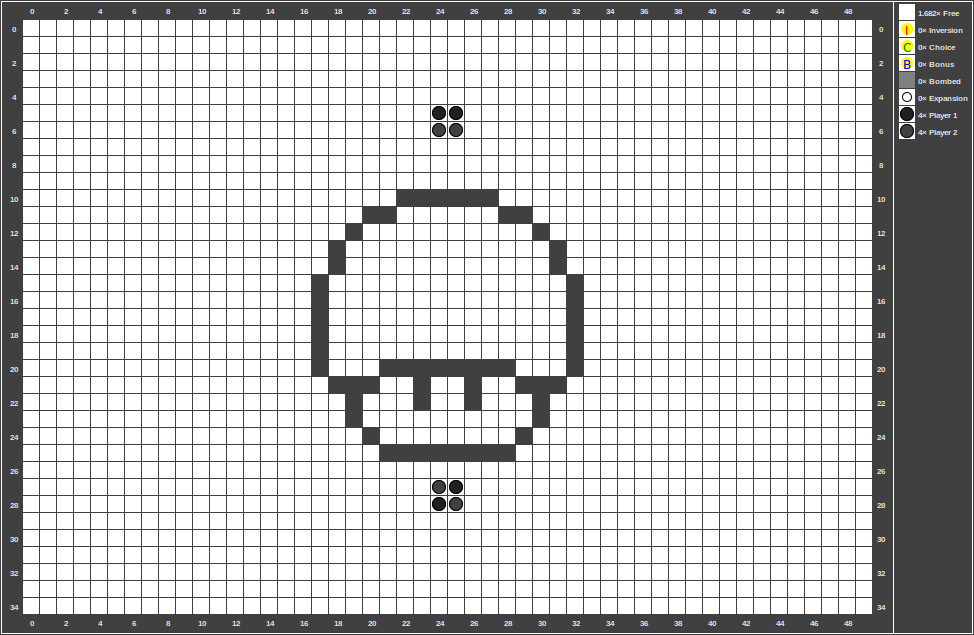
\includegraphics[width=0.5\linewidth]{pics/gamefield01.png}
	\captionof{figure}[Spielfeld 01]{Unbespieltes Spielfeld\footnotemark }
	\label{fig:reversi01}
\end{minipage}
\footnotetext{Diesem Spielfeld wurden noch keine Spieler zugewiesen (daher die dunklen Spielsteine)}

Nachdem das Spielt gestartet wurde und beide Spielphasen durchlaufen wurden, siegt schließlich der Spieler mit der Farbe rot.

%\vspace{1em}
%\begin{minipage}{\linewidth}
%	\centering
%	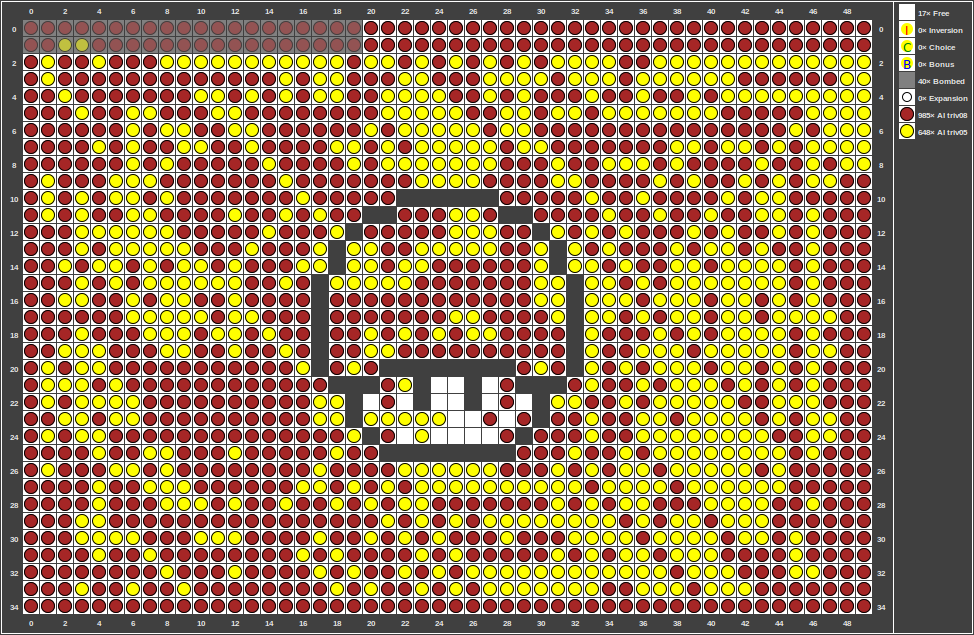
\includegraphics[width=0.5\linewidth]{pics/gamefield02.png}
%	\captionof{figure}[Spielfeld 02]{Finales Spielfeld\footnotemark }
%	\label{fig:reversi2}
%\end{minipage}
%\footnotetext{Das Spielfeld nach der Zug- und Bombenphase. Spieler rot gewinnt eindeutig.}

\subsection{Tabellen}
In diesem Abschnitt wird eine Tabelle (siehe Tabelle \ref{tab:beispiel}) dargestellt.

\vspace{1em}
\begin{table}[!h]
	\centering
	\begin{tabular}{|l|l|l|}
		\hline
		\textbf{Name} & \textbf{Name} & \textbf{Name}\\
		\hline
		1 & 2 & 3\\
		\hline
		4 & 5 & 6\\
		\hline
		7 & 8 & 9\\
		\hline
	\end{tabular}
	\caption{Beispieltabelle}
	\label{tab:beispiel}
\end{table}


\subsection{Auflistung}
Für Auflistungen wird die \texttt{enumerate}- oder \texttt{itemize}-Umgebung genutzt.

\begin{itemize}
	\item Nur
	\item ein
	\item Beispiel.
\end{itemize}

\subsection{Listings}
Zuletzt sehen Sie in Listing \ref{lst:maxTeilsumZweiD} ein Beispiel für das Einbinden von Quellcode mit Syntax-Highlighting.

\vspace{1em}
\lstinputlisting[caption=Brute Force-Ansatz für das MaxTeilsum2D-Problem, label=lst:maxTeilsumZweiD,basicstyle=\ttfamily\scriptsize]{code/maxTeilsum2DBruteForce.txt}

\subsection{Selbstgestaltete Abbildungen}
Mithilfe des Paketes \texttt{tikz} können sehr schöne Abbildungen (z.\,B.\ Automaten, Graphen etc.) direkt in \LaTeX generiert werden. Viele Beispiele dazu finden Sie auf folgender Webseite:\\[1em]
\hspace*{3cm}\url{http://www.texample.net/tikz/}.

\subsection{Tipps}
Die Literaturreferenzen (Bücher, Paper und Journals) und Internetquellen (Webseiten, Blogs etc.) befinden sich in der Datei \textit{literatur.bib}. Eine Buch- und eine Online-Quelle sind beispielhaft eingefügt.  %\cite{Bui2015AnalysisSecurity} 

Literatur und Quellen werden in zwei getrennte Verzeichnisse aufgeteilt. Als Unterscheidungsmerkmal dient bei den Quellen der Zusatz: \texttt{keywords = \{online\}}.

\pagebreak

% ----------------------------------------------------------------------------------------------------------
% Filter fuer Literatur und Quellen definieren
% ----------------------------------------------------------------------------------------------------------

%\defbibheading{Literatur}{\section*{Literaturverzeichnis}} 
\defbibheading{Quellen}{\section*{Quellenverzeichnis}} 
  
%\defbibfilter{Literatur}{\not\keyword{online}} 
%\defbibfilter{Quellen}{\keyword{online}} 


% ----------------------------------------------------------------------------------------------------------
% Literatur
% ----------------------------------------------------------------------------------------------------------
%\lhead{} 
%\rhead{Literaturverzeichnis} 

%\printbibliography[heading=Literatur,filter=Literatur] 

%\pagebreak


% ---------------------------------------------------------------------------------------------------------- 
% Quellen 
% ---------------------------------------------------------------------------------------------------------- 
\lhead{} 
\rhead{Quellenverzeichnis} 

%\printbibliography[title = {Quellenverzeichnis}, heading=Quellen] 
%\printbibliography[title = {Quellenverzeichnis},
\printbibliography[title = {Quellenverzeichnis}, heading=Quellen]

\pagebreak 

% ----------------------------------------------------------------------------------------------------------
% Anhang
% ----------------------------------------------------------------------------------------------------------
\pagenumbering{Roman}
\setcounter{page}{1}
\lhead{Anhang \thesection}

\begin{appendix}
\section*{Anhang}
\phantomsection
\addcontentsline{toc}{section}{Anhang}
\addtocontents{toc}{\vspace{-0.5em}}

Inhalt des beigefügten Datenträgers:
\begin{itemize}
  \item $\ldots$
  \item $\ldots$
\end{itemize}

\section{Domändenmodell}
Ein toller Anhang, der nicht nur als \glqq{}\emph{Müllhalde}\grqq{} genutzt wird, sondern in dem Bilder und Inhalte auch mit eigenen Worten erklärt werden und den man auch für sich alleine lesen kann. Es sollten auch Referenzen auf die zugehörige ausführliche Behandlung im Hauptteil inklusive Seitenangabe mit $\backslash$\texttt{pageref} gegeben werden.

\subsection*{Screenshot}
\label{app:screenshot}
Unterkategorie, die nicht im Inhaltsverzeichnis auftaucht.

\end{appendix}


\pagebreak


%\bibliographystyle{ieeetr}
%\bibliography{mendeley}
\end{document}

